%% March 2018
%DIF LATEXDIFF DIFFERENCE FILE
%DIF DEL ../g3_v2/coupling_v2.tex   Sun May 23 17:44:08 2021
%DIF ADD ../g3_v3/coupling_v3.tex   Sun May 23 17:27:52 2021
%%%%%%%%%%%%%%%%%%%%%%%%%%%%%%%%%%%%%%%%%%%%%%%%%%%%%%%%%%%%%%%%%%%%%%%%%%%%
% AGUJournalTemplate.tex: this template file is for articles formatted with LaTeX
%
% This file includes commands and instructions
% given in the order necessary to produce a final output that will
% satisfy AGU requirements, including customized APA reference formatting.
%
% You may copy this file and give it your
% article name, and enter your text.
%
%
% Step 1: Set the \documentclass
%
% There are two options for article format:
%
% PLEASE USE THE DRAFT OPTION TO SUBMIT YOUR PAPERS.
% The draft option produces double spaced output.
%

%% To submit your paper:
\documentclass[draft,linenumbers]{agujournal2018}
\usepackage{apacite}
\usepackage{url} %this package should fix any errors with URLs in refs.
%%%%%%%
% As of 2018 we recommend use of the TrackChanges package to mark revisions.
% The trackchanges package adds five new LaTeX commands:
%
%  \note[editor]{The note}
%  \annote[editor]{Text to annotate}{The note}
%  \add[editor]{Text to add}
%  \remove[editor]{Text to remove}
%  \change[editor]{Text to remove}{Text to add}
%
% complete documentation is here: http://trackchanges.sourceforge.net/
%%%%%%%


%% Enter journal name below.
%% Choose from this list of Journals:
%
% JGR: Atmospheres
% JGR: Biogeosciences
% JGR: Earth Surface
% JGR: Oceans
% JGR: Planets
% JGR: Solid Earth
% JGR: Space Physics
% Global Biogeochemical Cycles
% Geophysical Research Letters
% Paleoceanography and Paleoclimatology
% Radio Science
% Reviews of Geophysics
% Tectonics
% Space Weather
% Water Resources Research
% Geochemistry, Geophysics, Geosystems
% Journal of Advances in Modeling Earth Systems (JAMES)
% Earth's Future
% Earth and Space Science
% Geohealth
%
% ie, \journalname{Water Resources Research}

\journalname{Geochemistry, Geophysics, Geosystems}

% Pandoc citation processing
\newlength{\csllabelwidth}
\setlength{\csllabelwidth}{3em}
\newlength{\cslhangindent}
\setlength{\cslhangindent}{1.5em}
% for Pandoc 2.8 to 2.10.1
\newenvironment{cslreferences}%
  {}%
  {\par}
% For Pandoc 2.11+
\newenvironment{CSLReferences}[2] % #1 hanging-ident, #2 entry spacing
 {% don't indent paragraphs
  \setlength{\parindent}{0pt}
  % turn on hanging indent if param 1 is 1
  \ifodd #1 \everypar{\setlength{\hangindent}{\cslhangindent}}\ignorespaces\fi
  % set entry spacing
  \ifnum #2 > 0
  \setlength{\parskip}{#2\baselineskip}
  \fi
 }%
 {}
\usepackage{calc} % for calculating minipage widths
\newcommand{\CSLBlock}[1]{#1\hfill\break}
\newcommand{\CSLLeftMargin}[1]{\parbox[t]{\csllabelwidth}{#1}}
\newcommand{\CSLRightInline}[1]{\parbox[t]{\linewidth - \csllabelwidth}{#1}\break}
\newcommand{\CSLIndent}[1]{\hspace{\cslhangindent}#1}


\usepackage{booktabs}
\usepackage{soulutf8}
\usepackage{setspace}
\usepackage{caption}
\captionsetup[figure]{font={stretch=0.6, footnotesize}}
\usepackage{hyperref}
\usepackage{amsmath}
\usepackage{float}
\usepackage{longtable}
\usepackage{pdflscape}
\usepackage{threeparttable}
\def\tightlist{}
\usepackage{booktabs} %DIF > 
\usepackage{longtable} %DIF > 
\usepackage{array} %DIF > 
\usepackage{multirow} %DIF > 
\usepackage{wrapfig} %DIF > 
\usepackage{float} %DIF > 
\usepackage{colortbl} %DIF > 
\usepackage{pdflscape} %DIF > 
\usepackage{tabu} %DIF > 
\usepackage{threeparttable} %DIF > 
\usepackage{threeparttablex} %DIF > 
\usepackage[normalem]{ulem} %DIF > 
\usepackage{makecell} %DIF > 
\usepackage{xcolor} %DIF > 
%DIF PREAMBLE EXTENSION ADDED BY LATEXDIFF
%DIF CFONT PREAMBLE %DIF PREAMBLE
\RequirePackage{color}\definecolor{RED}{rgb}{1,0,0}\definecolor{BLUE}{rgb}{0,0,1} %DIF PREAMBLE
\DeclareOldFontCommand{\sf}{\normalfont\sffamily}{\mathsf} %DIF PREAMBLE
\providecommand{\DIFaddtex}[1]{{\protect\color{blue} \sf #1}} %DIF PREAMBLE
\providecommand{\DIFdeltex}[1]{{\protect\color{red} \scriptsize #1}} %DIF PREAMBLE
%DIF SAFE PREAMBLE %DIF PREAMBLE
\providecommand{\DIFaddbegin}{} %DIF PREAMBLE
\providecommand{\DIFaddend}{} %DIF PREAMBLE
\providecommand{\DIFdelbegin}{} %DIF PREAMBLE
\providecommand{\DIFdelend}{} %DIF PREAMBLE
\providecommand{\DIFmodbegin}{} %DIF PREAMBLE
\providecommand{\DIFmodend}{} %DIF PREAMBLE
%DIF FLOATSAFE PREAMBLE %DIF PREAMBLE
\providecommand{\DIFaddFL}[1]{\DIFadd{#1}} %DIF PREAMBLE
\providecommand{\DIFdelFL}[1]{\DIFdel{#1}} %DIF PREAMBLE
\providecommand{\DIFaddbeginFL}{} %DIF PREAMBLE
\providecommand{\DIFaddendFL}{} %DIF PREAMBLE
\providecommand{\DIFdelbeginFL}{} %DIF PREAMBLE
\providecommand{\DIFdelendFL}{} %DIF PREAMBLE
%DIF HYPERREF PREAMBLE %DIF PREAMBLE
\providecommand{\DIFadd}[1]{\texorpdfstring{\DIFaddtex{#1}}{#1}} %DIF PREAMBLE
\providecommand{\DIFdel}[1]{\texorpdfstring{\DIFdeltex{#1}}{}} %DIF PREAMBLE
%DIF LISTINGS PREAMBLE %DIF PREAMBLE
\RequirePackage{listings} %DIF PREAMBLE
\RequirePackage{color} %DIF PREAMBLE
\lstdefinelanguage{DIFcode}{ %DIF PREAMBLE
%DIF DIFCODE_CFONT %DIF PREAMBLE
  moredelim=[il][\color{red}\scriptsize]{\%DIF\ <\ }, %DIF PREAMBLE
  moredelim=[il][\color{blue}\sffamily]{\%DIF\ >\ } %DIF PREAMBLE
} %DIF PREAMBLE
\lstdefinestyle{DIFverbatimstyle}{ %DIF PREAMBLE
	language=DIFcode, %DIF PREAMBLE
	basicstyle=\ttfamily, %DIF PREAMBLE
	columns=fullflexible, %DIF PREAMBLE
	keepspaces=true %DIF PREAMBLE
} %DIF PREAMBLE
\lstnewenvironment{DIFverbatim}{\lstset{style=DIFverbatimstyle}}{} %DIF PREAMBLE
\lstnewenvironment{DIFverbatim*}{\lstset{style=DIFverbatimstyle,showspaces=true}}{} %DIF PREAMBLE
%DIF END PREAMBLE EXTENSION ADDED BY LATEXDIFF

\begin{document}

%% ------------------------------------------------------------------------ %%
%  Title
%
% (A title should be specific, informative, and brief. Use
% abbreviations only if they are defined in the abstract. Titles that
% start with general keywords then specific terms are optimized in
% searches)
%
%% ------------------------------------------------------------------------ %%

% Example: \title{This is a test title}

\title{Backarc lithospheric thickness and serpentine stability control
slab-mantle coupling depths in subduction zones}

%% ------------------------------------------------------------------------ %%
%
%  AUTHORS AND AFFILIATIONS
%
%% ------------------------------------------------------------------------ %%

% Authors are individuals who have significantly contributed to the
% research and preparation of the article. Group authors are allowed, if
% each author in the group is separately identified in an appendix.)

% List authors by first name or initial followed by last name and
% separated by commas. Use \affil{} to number affiliations, and
% \thanks{} for author notes.
% Additional author notes should be indicated with \thanks{} (for
% example, for current addresses).

% Example: \authors{A. B. Author\affil{1}\thanks{Current address, Antartica}, B. C. Author\affil{2,3}, and D. E.
% Author\affil{3,4}\thanks{Also funded by Monsanto.}}

\authors{
Buchanan C. Kerswell
\affil{1}
Matthew J. Kohn
\affil{1}
Taras V. Gerya
\affil{2}
}


% \affiliation{1}{First Affiliation}
% \affiliation{2}{Second Affiliation}
% \affiliation{3}{Third Affiliation}
% \affiliation{4}{Fourth Affiliation}

\affiliation{1}{Department of Geosicences, Boise State University,
Boise, ID 83725}
\affiliation{2}{Department of Earth Sciences, ETH-Zurich, Sonneggstrasse
5, Zurich 8092, Switzerland}
%(repeat as many times as is necessary)

%% Corresponding Author:
% Corresponding author mailing address and e-mail address:

% (include name and email addresses of the corresponding author.  More
% than one corresponding author is allowed in this LaTeX file and for
% publication; but only one corresponding author is allowed in our
% editorial system.)

% Example: \correspondingauthor{First and Last Name}{email@address.edu}
\correspondingauthor{Buchanan C.
Kerswell}{\href{mailto:buchanankerswell@u.boisestate.edu}{\nolinkurl{buchanankerswell@u.boisestate.edu}}}

%% Keypoints, final entry on title page.

%  List up to three key points (at least one is required)
%  Key Points summarize the main points and conclusions of the article
%  Each must be 100 characters or less with no special characters or punctuation

% Example:
% \begin{keypoints}
% \item	List up to three key points (at least one is required)
% \item	Key Points summarize the main points and conclusions of the article
% \item	Each must be 100 characters or less with no special characters or punctuation
% \end{keypoints}

\begin{keypoints}
\item The depths of antigorite destabilization and mechanical coupling
are primarily dependent on backarc lithospheric thickness
\item Coupling depths in natural subduction zones can be predicted given
slab age, convergence velocity, and backarc lithospheric thickness
\item Consistently high backarc heat flow in natural subduction zones
may indicate a common depth of mechanical coupling globally at ca. 82
\(km\)
\end{keypoints}

%% ------------------------------------------------------------------------ %%
%
%  ABSTRACT
%
% A good abstract will begin with a short description of the problem
% being addressed, briefly describe the new data or analyses, then
% briefly states the main conclusion(s) and how they are supported and
% uncertainties.
%% ------------------------------------------------------------------------ %%

%% \begin{abstract} starts the second page

\begin{abstract}
A key feature of subduction zone geodynamics and thermal structure is
the point at which the slab and mantle mechanically couple. This point
defines the depth at which traction between slab and mantle begins to
drive mantle wedge circulation and also corresponds with a rapid
increase in temperature along the slab-mantle interface. Here we
consider the effects of the backarc thermal structure and slab thermal
parameter on coupling depth using two-dimensional thermomechanical
models of oceanic-continental convergent margins. Coupling depth is
strongly correlated with backarc lithospheric thickness, and weakly
correlated with slab thermal parameter. Slab-mantle coupling becomes
significant where weak, hydrous antigorite reacts to form strong,
anhydrous olivine and pyroxene along the slab-mantle interface. Highly
efficient (predominantly advective) heat transfer in the asthenospheric
mantle wedge and inefficient (predominantly conductive) heat transfer in
the lithospheric mantle wedge results in competing feedbacks that
stabilize the antigorite-out reaction at depths determined primarily by
the mechanical thickness of the backarc lithosphere. For subduction zone
segments where backarc lithospheric thickness can be inverted from
surface heat flow, our results provide a regression model that can be
applied with slab thermal parameter to predict coupling depth.
Consistently high backarc heat flow in circum-Pacific subduction zones
suggests uniformly thin overriding plates likely regulated by
lithospheric erosion caused by hydration and melting processes under
volcanic arcs. This may also explain a common depth of slab-mantle
coupling globally.
\end{abstract}
\noindent{\bf Plain language summary}\vskip-\parskip

\noindent{Subduction is a process where two semi-rigid tectonic plates
of Earth's outer shell converge, and one dives beneath the other into
the mantle. Subduction zones produce the world's largest earthquakes and
form new crust through volcanism. Understanding earthquakes and
volcanism requires understanding how the two plates move with respect to
each other. With increasing depth, the sinking plate transitions from
sliding past the overriding plate to ``gripping'' the base of the
overriding plate. This gripping (coupling) reduces earthquakes and
causes warm rock to flow upwards, enabling volcanism. We used
two-dimensional computer simulations of subduction to test what controls
the depth of coupling between the plates. We found that coupling depth
is primarily controlled by the thickness of the overriding plate and
provide an equation to predict coupling depth in natural subduction
zones. Overriding plates in subduction zones worldwide appear to have
similar thicknesses, so coupling depths are also predicted to be
similar. We do not yet fully understand why the overriding plates are
uniformly thin globally, but perhaps this is related to hydration and
melting under volcanic arcs.}
\vskip18pt
\hypertarget{introduction}{%
\section{Introduction}\label{introduction}}

The thermal structure of subduction zones strongly depends on the depth
where the subducting slab and overlying mantle transition from
mechanically decoupled (moving differentially with respect to each
other) to mechanically coupled (moving with the same local velocity,
\protect\hyperlink{ref-Furukawa1993}{Furukawa, 1993};
\protect\hyperlink{ref-Peacock1994}{Peacock et al., 1994};
\protect\hyperlink{ref-Wada2008}{Wada et al., 2008}). Coupling drives
mantle wedge circulation, and the decoupling-coupling transition defines
a rapid increase in temperature along the top of the subducting slab
(\protect\hyperlink{ref-Peacock1996}{Peacock, 1996}). Based on many
observations, the depth of slab-mantle coupling has been inferred from
numerical models to occur at 70-80 \(km\) depth, essentially independent
of other parameters including slab age, convergence velocity, and
subduction geometry (\protect\hyperlink{ref-Furukawa1993}{Furukawa,
1993}; \protect\hyperlink{ref-Wada2008}{Wada et al., 2008};
\protect\hyperlink{ref-Wada2009}{Wada \& Wang, 2009}). It is significant
that modern subduction zones appear to achieve similar depths of
coupling despite their different physical characteristics.

A prescribed slab-mantle coupling depth of 70-80 \(km\) has been used as
a physical condition in many thermomechanical models (e.g.,
\protect\hyperlink{ref-Abers2017}{Abers et al., 2017};
\protect\hyperlink{ref-Currie2004}{Currie et al., 2004};
\protect\hyperlink{ref-Gao2014}{Gao \& Wang, 2014};
\protect\hyperlink{ref-Syracuse2010}{Syracuse et al., 2010};
\protect\hyperlink{ref-VanKeken2011}{van Keken et al., 2011},
\protect\hyperlink{ref-VanKeken2018}{2018};
\protect\hyperlink{ref-Wada2012}{Wada et al., 2012};
\protect\hyperlink{ref-Wilson2014}{Wilson et al., 2014}), although
different coupling depths apply in other studies (e.g.~40-56 \(km\),
\protect\hyperlink{ref-England2010}{England \& Katz, 2010};
\protect\hyperlink{ref-Peacock1996}{Peacock, 1996}). A common coupling
depth is attractive for at least two reasons: Firstly, it helps explain
the relatively narrow range of sub-arc slab depths
(\protect\hyperlink{ref-England2004}{England et al., 2004};
\protect\hyperlink{ref-Syracuse2006}{Syracuse \& Abers, 2006}) as
mechanical coupling is expected to be closely associated with the onset
of flux melting. Secondly, since mechanical coupling is required to
detach and recover rocks from the down-going slab
(\protect\hyperlink{ref-Agard2016}{Agard et al., 2016}), a common depth
of coupling may also help explain why the maximum pressures recorded by
subducted oceanic material worldwide is ca. 2.3-2.5 \(GPa\) (roughly 80
\(km\), \protect\hyperlink{ref-Agard2009}{Agard et al., 2009}).

Beyond playing a crucial role in subduction zone thermal structure, the
location and extent of mechanical coupling along the slab-mantle
interface is implicated in a myriad of subduction zone geodynamics
(seismicity, metamorphism, volatile fluxes into the mantle wedge,
volcanism, and plate motions, e.g.,
\protect\hyperlink{ref-Cizkova2013}{Čížková \& Bina, 2013};
\protect\hyperlink{ref-Gao2017}{Gao \& Wang, 2017};
\protect\DIFaddbegin \hyperlink{ref-Gonzalez2016}{Gonzalez et al., 2016}\DIFadd{;
}\protect\DIFaddend \hyperlink{ref-Grove2012}{Grove et al., 2012};
\protect\hyperlink{ref-Hacker2003}{Hacker et al., 2003};
\protect\hyperlink{ref-Peacock1990}{Peacock, 1990},
\protect\hyperlink{ref-Peacock1991}{1991},
\protect\hyperlink{ref-Peacock1993}{1993},
\protect\hyperlink{ref-Peacock1996}{1996};
\protect\hyperlink{ref-Peacock1999a}{Peacock \& Hyndman, 1999};
\protect\hyperlink{ref-VanKeken2011}{van Keken et al., 2011}).
Consequently, the mechanics of coupling have been extensively studied
and discussed. Coupling fundamentally depends on the strength
(viscosity) of materials above, within, and below the slab-mantle
interface. In general, high water fluxes due to compaction and
dehydration of clays and other hydrous minerals in the shallow forearc
mantle wedge, coupled with increases in pressure and temperature, form
layers of low viscosity sheet silicates---especially talc and
serpentine---that inhibit transmission of shear stress from the slab to
the mantle wedge (\protect\hyperlink{ref-Peacock1999a}{Peacock \&
Hyndman, 1999}). The lack of traction along the interface combined with
cooling from the subducting slab surface ensures the shallow mantle
wedge remains cold and rigid. Experimentally determined flow laws (e.g.,
\protect\hyperlink{ref-Agard2016}{Agard et al., 2016}), petrologic
observations (e.g., \protect\hyperlink{ref-Agard2016}{Agard et al.,
2016}), and geophysical observations (e.g.,
\protect\hyperlink{ref-Gao2014}{Gao \& Wang, 2014};
\protect\hyperlink{ref-Peacock1999a}{Peacock \& Hyndman, 1999}) all
support the plausibility of this conceptual model of subduction
interface behavior.

Here we focus on two fundamental questions: 1) What controls the depth
of slab-mantle mechanical coupling? 2) How does coupling depth change
through time? To address these questions, we use two-dimensional
thermomechanical models of subduction to investigate potential
correlations between the slab-mantle coupling depth, backarc
lithospheric thickness (inverted from backarc heat flow), and slab
thermal parameter (\(\Phi\)). \protect\hyperlink{ref-Wada2009}{Wada \&
Wang} (\protect\hyperlink{ref-Wada2009}{2009}) previously investigated
steady-state slab-mantle coupling depths by modelling 17 active
subduction zones. Among other parameters, their models specified
convergence rate, subduction geometry, thermal structure of incoming and
overriding plate, and degree of coupling vs.~decoupling with depth along
the subduction interface. Notably, their models prescribed the
mechanical coupling depth for each subduction zone, did not include
mineral reactions that might influence rheologies, and discriminated the
best-fit depth based on observed fore-arc heat flow. In our models, we
also specify horizontal convergence velocity and thermal structure of
the incoming and overriding plates, as one would for modeling a modern
system. However, the geometry of the subduction system and (most
importantly) the point of mechanical coupling are allowed to evolve
independently until they reach steady state. That is, the coupling depth
in each of our models is not a fully determined feature but rather a
spontaneous model outcome. As in other previous studies (e.g.,
\protect\hyperlink{ref-Ruh2015}{Ruh et al., 2015}), we also include the
rheological effect of the dehydration reaction
\(antigorite \allowbreak \Leftrightarrow olivine + orthopyroxene + H_{2}O\),
which drives mechanical coupling by an abrupt viscosity increase with
antigorite loss. The position of this reaction along the subduction
interface determines the coupling depth.

We quantify the effects of \(\Phi\) and backarc lithospheric thickness
on the depth of this reaction using linear regression. We then visualize
thermal feedbacks within the system in terms of the distributions of
temperature, viscosity, and mantle flow velocity. Last, we discuss how
feedbacks stabilize the coupling depth through millions of years of
subduction.

\hypertarget{numerical-modelling-methods}{%
\section{Numerical Modelling
Methods}\label{numerical-modelling-methods}}

Our models simulated converging oceanic-continental plates, where an
ocean basin is being consumed by subduction at a continental margin
(Figure~\ref{fig:init}). The initial conditions were modified from
previous modeling studies of active margins
(\protect\hyperlink{ref-Gorczyk2007}{Gorczyk et al., 2007};
\protect\hyperlink{ref-Sizova2010}{Sizova et al., 2010}), although
slab-mantle coupling was not the focus of their studies. Our approach
was to use identical material properties (Tables \ref{tab:materials},
\ref{tab:melts}), rheologic model, and hydration/melt model (see
Appendix) as \protect\hyperlink{ref-Sizova2010}{Sizova et al.}
(\protect\hyperlink{ref-Sizova2010}{2010}). Our version differed from
\protect\hyperlink{ref-Sizova2010}{Sizova et al.}
(\protect\hyperlink{ref-Sizova2010}{2010}) in its initial setup, overall
dimension, resolution, the shape of the continental geotherm, the slab
dehydration model, and the left boundary condition (origin of the
subducting slab). These differences are outlined below. Sixty-four
models were constructed with varying convergence rate, subducting plate
age, and the lithospheric thickness of the overriding plate
(Figure~\ref{fig:params}).

\begin{figure}[h]

{\centering 
\includegraphics[width=1\linewidth,]{figs/fig1} 

}

\caption{Initial model configuration and boundary conditions. (a) A free sedimentation/erosion boundary at the surface is maintained by implementing a layer of "sticky" air and water, and an infinite-like open boundary at the bottom allows for slab penetration. The left and right boundaries are free slip and insulating. The initial material distribution includes 7 $km$ of oceanic crust (2 $km$ basalt, 5 $km$ gabbro), 1 $km$ of oceanic sediments, and 35 $km$ of continental crust, thinning ocean-ward. (b) Oceanic lithosphere is continually created at the left boundary. The oceanic geotherm is calculated using a half-space cooling model and the continental geotherm is calculated using a one-dimensional steady-state conductive cooling model to 1300 $^{\circ}C$. The base of the lithosphere is defined mechanically through visualization of viscosity and generally coincides with the 1100 $^{\circ}C$ isotherm ($z_{1100}$). (c) The oceanic crust is bent under loading from passive margin sediments, and a weak zone extends from the deflected oceanic crust, through the lithosphere, to help induce subduction. Convergence velocities are imposed at stationary regions far from the trench. Rock type colors are given in Table \ref{tab:rock.type}.}\label{fig:init}
\end{figure}

\begin{landscape}\begin{table}

\caption{\label{tab:materials}Rheologic parameters used in numerical experiments}
\centering
\resizebox{\linewidth}{!}{
\begin{threeparttable}
\begin{tabular}[t]{llllllllllllllllll}
\toprule
\multicolumn{1}{c}{Material} & \multicolumn{1}{c}{Flow Law} & \multicolumn{1}{c}{$h$} & \multicolumn{1}{c}{$m$} & \multicolumn{1}{c}{$n$} & \multicolumn{1}{c}{$A$} & \multicolumn{1}{c}{$A_{diff}$} & \multicolumn{1}{c}{$A_{disl}$} & \multicolumn{1}{c}{$V$} & \multicolumn{1}{c}{$V_{diff}$} & \multicolumn{1}{c}{$V_{disl}$} & \multicolumn{1}{c}{$E$} & \multicolumn{1}{c}{$E_{diff}$} & \multicolumn{1}{c}{$E_{disl}$} & \multicolumn{1}{c}{$\sigma_{cr}$} & \multicolumn{1}{c}{$C$} & \multicolumn{1}{c}{$\mu_0$} & \multicolumn{1}{c}{$\mu_1$} \\
\cmidrule(l{3pt}r{3pt}){1-1} \cmidrule(l{3pt}r{3pt}){2-2} \cmidrule(l{3pt}r{3pt}){3-3} \cmidrule(l{3pt}r{3pt}){4-4} \cmidrule(l{3pt}r{3pt}){5-5} \cmidrule(l{3pt}r{3pt}){6-6} \cmidrule(l{3pt}r{3pt}){7-7} \cmidrule(l{3pt}r{3pt}){8-8} \cmidrule(l{3pt}r{3pt}){9-9} \cmidrule(l{3pt}r{3pt}){10-10} \cmidrule(l{3pt}r{3pt}){11-11} \cmidrule(l{3pt}r{3pt}){12-12} \cmidrule(l{3pt}r{3pt}){13-13} \cmidrule(l{3pt}r{3pt}){14-14} \cmidrule(l{3pt}r{3pt}){15-15} \cmidrule(l{3pt}r{3pt}){16-16} \cmidrule(l{3pt}r{3pt}){17-17} \cmidrule(l{3pt}r{3pt}){18-18}
 &  & $m$ &  &  & $Pa^n s$ & $s^{-1}$ & $s^{-1}$ & $\frac{J}{Pa\cdot mol}$ & $\frac{J}{Pa\cdot mol}$ & $\frac{J}{Pa\cdot mol}$ & $\frac{J}{mol}$ & $\frac{J}{mol}$ & $\frac{J}{mol}$ & $Pa$ & $Pa$ &  & \\
\midrule
Felsic sediments & Wet quartzite &  &  & 2.3 & 1.97e+17 &  &  & 3e-06 &  &  & 1.54e+05 &  &  & 3e+04 & 1e+06 & 0.2 & 0.1\\
Felsic crust & Wet quartzite &  &  & 2.3 & 1.97e+17 &  &  & 3e-06 &  &  & 1.54e+05 &  &  & 3e+04 & 1e+06 & 0.6 & 0.3\\
Oceanic crust & Plag An$_{75}$ &  &  & 3.2 & 4.8e+22 &  &  & 8e-06 &  &  & 2.38e+05 &  &  & 3e+04 & 3e+05 & 0.6 & 0.2\\
Dry mantle & Dry olivine & 0.001 & 2.5 & 3.5 &  & 8.7e+15 & 3.5e+22 &  & 4e-06 & 2e-05 &  & 3e+05 & 5.4e+05 &  & 1e+06 & 0.6 & 0.3\\
Hydrated mantle & Wet olivine & 0.001 & 2.5 & 3 &  & 5.3e+15 & 2e+18 &  & 4e-06 & 1e-05 &  & 2.4e+05 & 4.3e+05 &  & 1e+06 & 0.6 & 0.3\\
\addlinespace
Serpentinized mantle & Serpentine &  &  & 3.8 & 3.21e+36 &  &  & 3.2e-06 &  &  & 8.9e+03 &  &  & 3e+06 & 1e+06 & 0.2 & 0.1\\
\midrule
Reference$^1$ & b, c, d & d & d & b, c, d & b, c & d & d & b, c & d & d & b, c & d & d & b, c & a &  & \\
\bottomrule
\end{tabular}
\begin{tablenotes}
\item $h$=grain size, $m$=grain size exponent, $n$=stress exponent, $A$=material constant, $V$=activation volume, $E$=activation energy, $\sigma_{cr}$=critical stress for dislocation creep, $C$=compressive strength at $P$=0, $\mu_{0,1}$=initial and final internal friction coefficient, $\mu_0=\mu_1=0$ for melt-bearing rocks
\item[1] a=Turcotte \& Schubert (2002), b=Ranalli (1995), c=Hilairet et al. (2007), d=Karato \& Wu (1993)
\end{tablenotes}
\end{threeparttable}}
\end{table}
\end{landscape}

\hypertarget{initial-setup-and-boundary-conditions}{%
\subsection{Initial setup and boundary
conditions}\label{initial-setup-and-boundary-conditions}}

Our two-dimensional model was 2000 \(km\) wide and 300 \(km\) deep
(Figure~\ref{fig:init}). In the model domain, three governing equations
of heat transport, motion, and continuity were discretized and solved
using a conservative finite-difference with marker-in-cell approach on a
fully staggered grid (code: \texttt{I2VIS}) as outlined in
\protect\hyperlink{ref-Gerya2003}{Gerya \& Yuen}
(\protect\hyperlink{ref-Gerya2003}{2003}). The model resolution was
non-uniform with higher resolution (1 \(km\) x 1 \(km\)) in a 600 \(km\)
wide area surrounding the contact between the ocean basin and
continental margin and gradually changing to lower resolution (5 \(km\)
x 1 \(km\), x- and z-directions, respectively) outside of this area. The
left and right boundaries were free-slip and thermally insulating
(Figure~\ref{fig:init}a, b). The implementation of ``sticky'' air and
water allowed for a free topographical surface with a simple linear
sedimentation and erosion model. The lower boundary was open to allow
for slab penetration and spontaneous slab motion
(\protect\hyperlink{ref-Burg2005}{Burg \& Gerya, 2005}).

\begin{table}
\DIFdelbeginFL %DIFDELCMD < \caption{%
{%DIFAUXCMD
%DIFDELCMD < \label{tab:rock.type}%%%
\DIFdelFL{Key for rock types used in model visualizations}}
%DIFAUXCMD
\DIFdelendFL 

\DIFaddbeginFL \caption{\label{tab:rock.type}\DIFaddFL{Key for rock types used in model visualizations}}
\DIFaddendFL \centering
\fontsize{8}{10}\selectfont
\begin{tabular}[t]{rl}
\toprule
Number & Rock Type\\
\midrule
\DIFdelbeginFL \DIFdelFL{0 }\DIFdelendFL \DIFaddbeginFL \DIFaddFL{1 }\DIFaddendFL & Air\\
\DIFdelbeginFL \DIFdelFL{1 }\DIFdelendFL \DIFaddbeginFL \DIFaddFL{2 }\DIFaddendFL & Water\\
\DIFdelbeginFL \DIFdelFL{2 }%DIFDELCMD < & %%%
\DIFdelFL{Sediments}%DIFDELCMD < \\
%DIFDELCMD < %%%
\DIFdelFL{3 }%DIFDELCMD < & %%%
\DIFdelFL{Sediments}%DIFDELCMD < \\
%DIFDELCMD < %%%
\DIFdelendFL 4 & Sediments\\
\DIFdelbeginFL %DIFDELCMD < \addlinespace
%DIFDELCMD < %%%
\DIFdelendFL 5 & \DIFdelbeginFL \DIFdelFL{Felsic Crust}\DIFdelendFL \DIFaddbeginFL \DIFaddFL{Sediments}\DIFaddendFL \\
6 & Felsic Crust\\
\DIFaddbeginFL %DIFDELCMD < \addlinespace
\DIFaddendFL 7 & \DIFdelbeginFL \DIFdelFL{Basalt}\DIFdelendFL \DIFaddbeginFL \DIFaddFL{Felsic Crust}\DIFaddendFL \\
8 & \DIFdelbeginFL \DIFdelFL{Gabbro}\DIFdelendFL \DIFaddbeginFL \DIFaddFL{Basalt}\DIFaddendFL \\
9 & \DIFdelbeginFL \DIFdelFL{Dry Mantle}\DIFdelendFL \DIFaddbeginFL \DIFaddFL{Gabbro}\DIFaddendFL \\
\DIFdelbeginFL %DIFDELCMD < \addlinespace
%DIFDELCMD < %%%
\DIFdelendFL 10 & Dry Mantle\\
11 & \DIFdelbeginFL \DIFdelFL{Hydrated Mantle}%DIFDELCMD < \\
%DIFDELCMD < %%%
\DIFdelFL{12 }%DIFDELCMD < & %%%
\DIFdelFL{Depleted Mantle}%DIFDELCMD < \\
%DIFDELCMD < %%%
\DIFdelFL{13 }%DIFDELCMD < & %%%
\DIFdelFL{Serpentinized Mantle}%DIFDELCMD < \\
%DIFDELCMD < %%%
\DIFdelFL{14 }%DIFDELCMD < & %%%
\DIFdelFL{Mantle Residue}%DIFDELCMD < \\
%DIFDELCMD < \addlinespace
%DIFDELCMD < %%%
\DIFdelFL{15 }%DIFDELCMD < & %%%
\DIFdelFL{Quenched Sediments}%DIFDELCMD < \\
%DIFDELCMD < %%%
\DIFdelFL{16 }%DIFDELCMD < & %%%
\DIFdelFL{Quenced Basalt from Basalt}%DIFDELCMD < \\
%DIFDELCMD < \bottomrule
%DIFDELCMD < \end{tabular}
%DIFDELCMD < \centering
%DIFDELCMD < \begin{tabular}[t]{rl}
%DIFDELCMD < \toprule
%DIFDELCMD < %%%
\DIFdelFL{Number }%DIFDELCMD < & %%%
\DIFdelFL{Rock Type}%DIFDELCMD < \\
%DIFDELCMD < \midrule
%DIFDELCMD < %%%
\DIFdelFL{17 }%DIFDELCMD < & %%%
\DIFdelFL{Quenched Basalt from Gabbro}%DIFDELCMD < \\
%DIFDELCMD < %%%
\DIFdelFL{18 }%DIFDELCMD < & %%%
\DIFdelFL{Quenched Basalt from Mantle}%DIFDELCMD < \\
%DIFDELCMD < %%%
\DIFdelFL{19 }%DIFDELCMD < & %%%
\DIFdelFL{Dry Lower-Density }\DIFdelendFL \DIFaddbeginFL \DIFaddFL{Dry }\DIFaddendFL Mantle\\
\DIFdelbeginFL \DIFdelFL{23 }%DIFDELCMD < & %%%
\DIFdelFL{Molten Sediments}%DIFDELCMD < \\
%DIFDELCMD < %%%
\DIFdelFL{24 }%DIFDELCMD < & %%%
\DIFdelFL{Molten Sediments}%DIFDELCMD < \\
%DIFDELCMD < %%%
\DIFdelendFL %DIFDELCMD < \addlinespace
\DIFdelbeginFL \DIFdelFL{25 }\DIFdelendFL \DIFaddbeginFL \DIFaddFL{12 }\DIFaddendFL & \DIFdelbeginFL \DIFdelFL{Molten Felsic Crust}%DIFDELCMD < \\
%DIFDELCMD < %%%
\DIFdelFL{26 }%DIFDELCMD < & %%%
\DIFdelFL{Molten Felsic Crust}%DIFDELCMD < \\
%DIFDELCMD < %%%
\DIFdelFL{27 }%DIFDELCMD < & %%%
\DIFdelFL{Molten Basalt}%DIFDELCMD < \\
%DIFDELCMD < %%%
\DIFdelFL{28 }%DIFDELCMD < & %%%
\DIFdelFL{Molten Basalt}%DIFDELCMD < \\
%DIFDELCMD < %%%
\DIFdelFL{29 }%DIFDELCMD < & %%%
\DIFdelFL{Molten Dry Mantle}%DIFDELCMD < \\
%DIFDELCMD < \addlinespace
%DIFDELCMD < %%%
\DIFdelFL{30 }%DIFDELCMD < & %%%
\DIFdelFL{Molten Dry Mantle}%DIFDELCMD < \\
%DIFDELCMD < %%%
\DIFdelFL{31 }%DIFDELCMD < & %%%
\DIFdelFL{Molten Dry Mantle}%DIFDELCMD < \\
%DIFDELCMD < %%%
\DIFdelFL{34 }%DIFDELCMD < & %%%
\DIFdelFL{Molten }\DIFdelendFL Hydrated Mantle\\
\DIFdelbeginFL \DIFdelFL{35 }\DIFdelendFL \DIFaddbeginFL \DIFaddFL{14 }\DIFaddendFL & \DIFdelbeginFL \DIFdelFL{Molten Quenched Sediments}%DIFDELCMD < \\
%DIFDELCMD < %%%
\DIFdelFL{36 }%DIFDELCMD < & %%%
\DIFdelFL{Molten Basalt from Basalt}%DIFDELCMD < \\
%DIFDELCMD < \addlinespace
%DIFDELCMD < %%%
\DIFdelFL{37 }%DIFDELCMD < & %%%
\DIFdelFL{Molten Basalt from Gabbro}%DIFDELCMD < \\
%DIFDELCMD < %%%
\DIFdelFL{38 }%DIFDELCMD < & %%%
\DIFdelFL{Molten Basalt from }\DIFdelendFL \DIFaddbeginFL \DIFaddFL{Serpentinized }\DIFaddendFL Mantle\\
\bottomrule
\end{tabular}
\end{table}

A horizontal convergence force was applied to both plates in a
rectangular region far from the continental margin
(Figure~\ref{fig:init}c). An initial weak layer cutting the lithosphere
permitted subduction to initiate. The rectangular convergence regions
prescribed inside the plates applied constant horizontal velocities
without deforming the lithosphere by maintaining constant viscosities of
\(\eta = 10^{25}~Pa\cdot s\). The subduction angle was not prescribed
and was governed by the free-motion of the sinking slab. Similarly,
subduction velocity can vary with time in response to extension or
shortening of the overriding plate. Therefore, we calculated the slab
thermal parameter (\(\Phi\)) for the initial conditions as the product
of the horizontal convergence velocity (\(km/Ma\)) and the slab age
(\(Ma\), c.f. \protect\hyperlink{ref-McKenzie1969}{McKenzie, 1969}). We
use \(\Phi\)/100 as it is commonly presented in the literature to reduce
the thermal parameter to convenient values (Figure~\ref{fig:params}a).

\begin{figure}[h]

{\centering 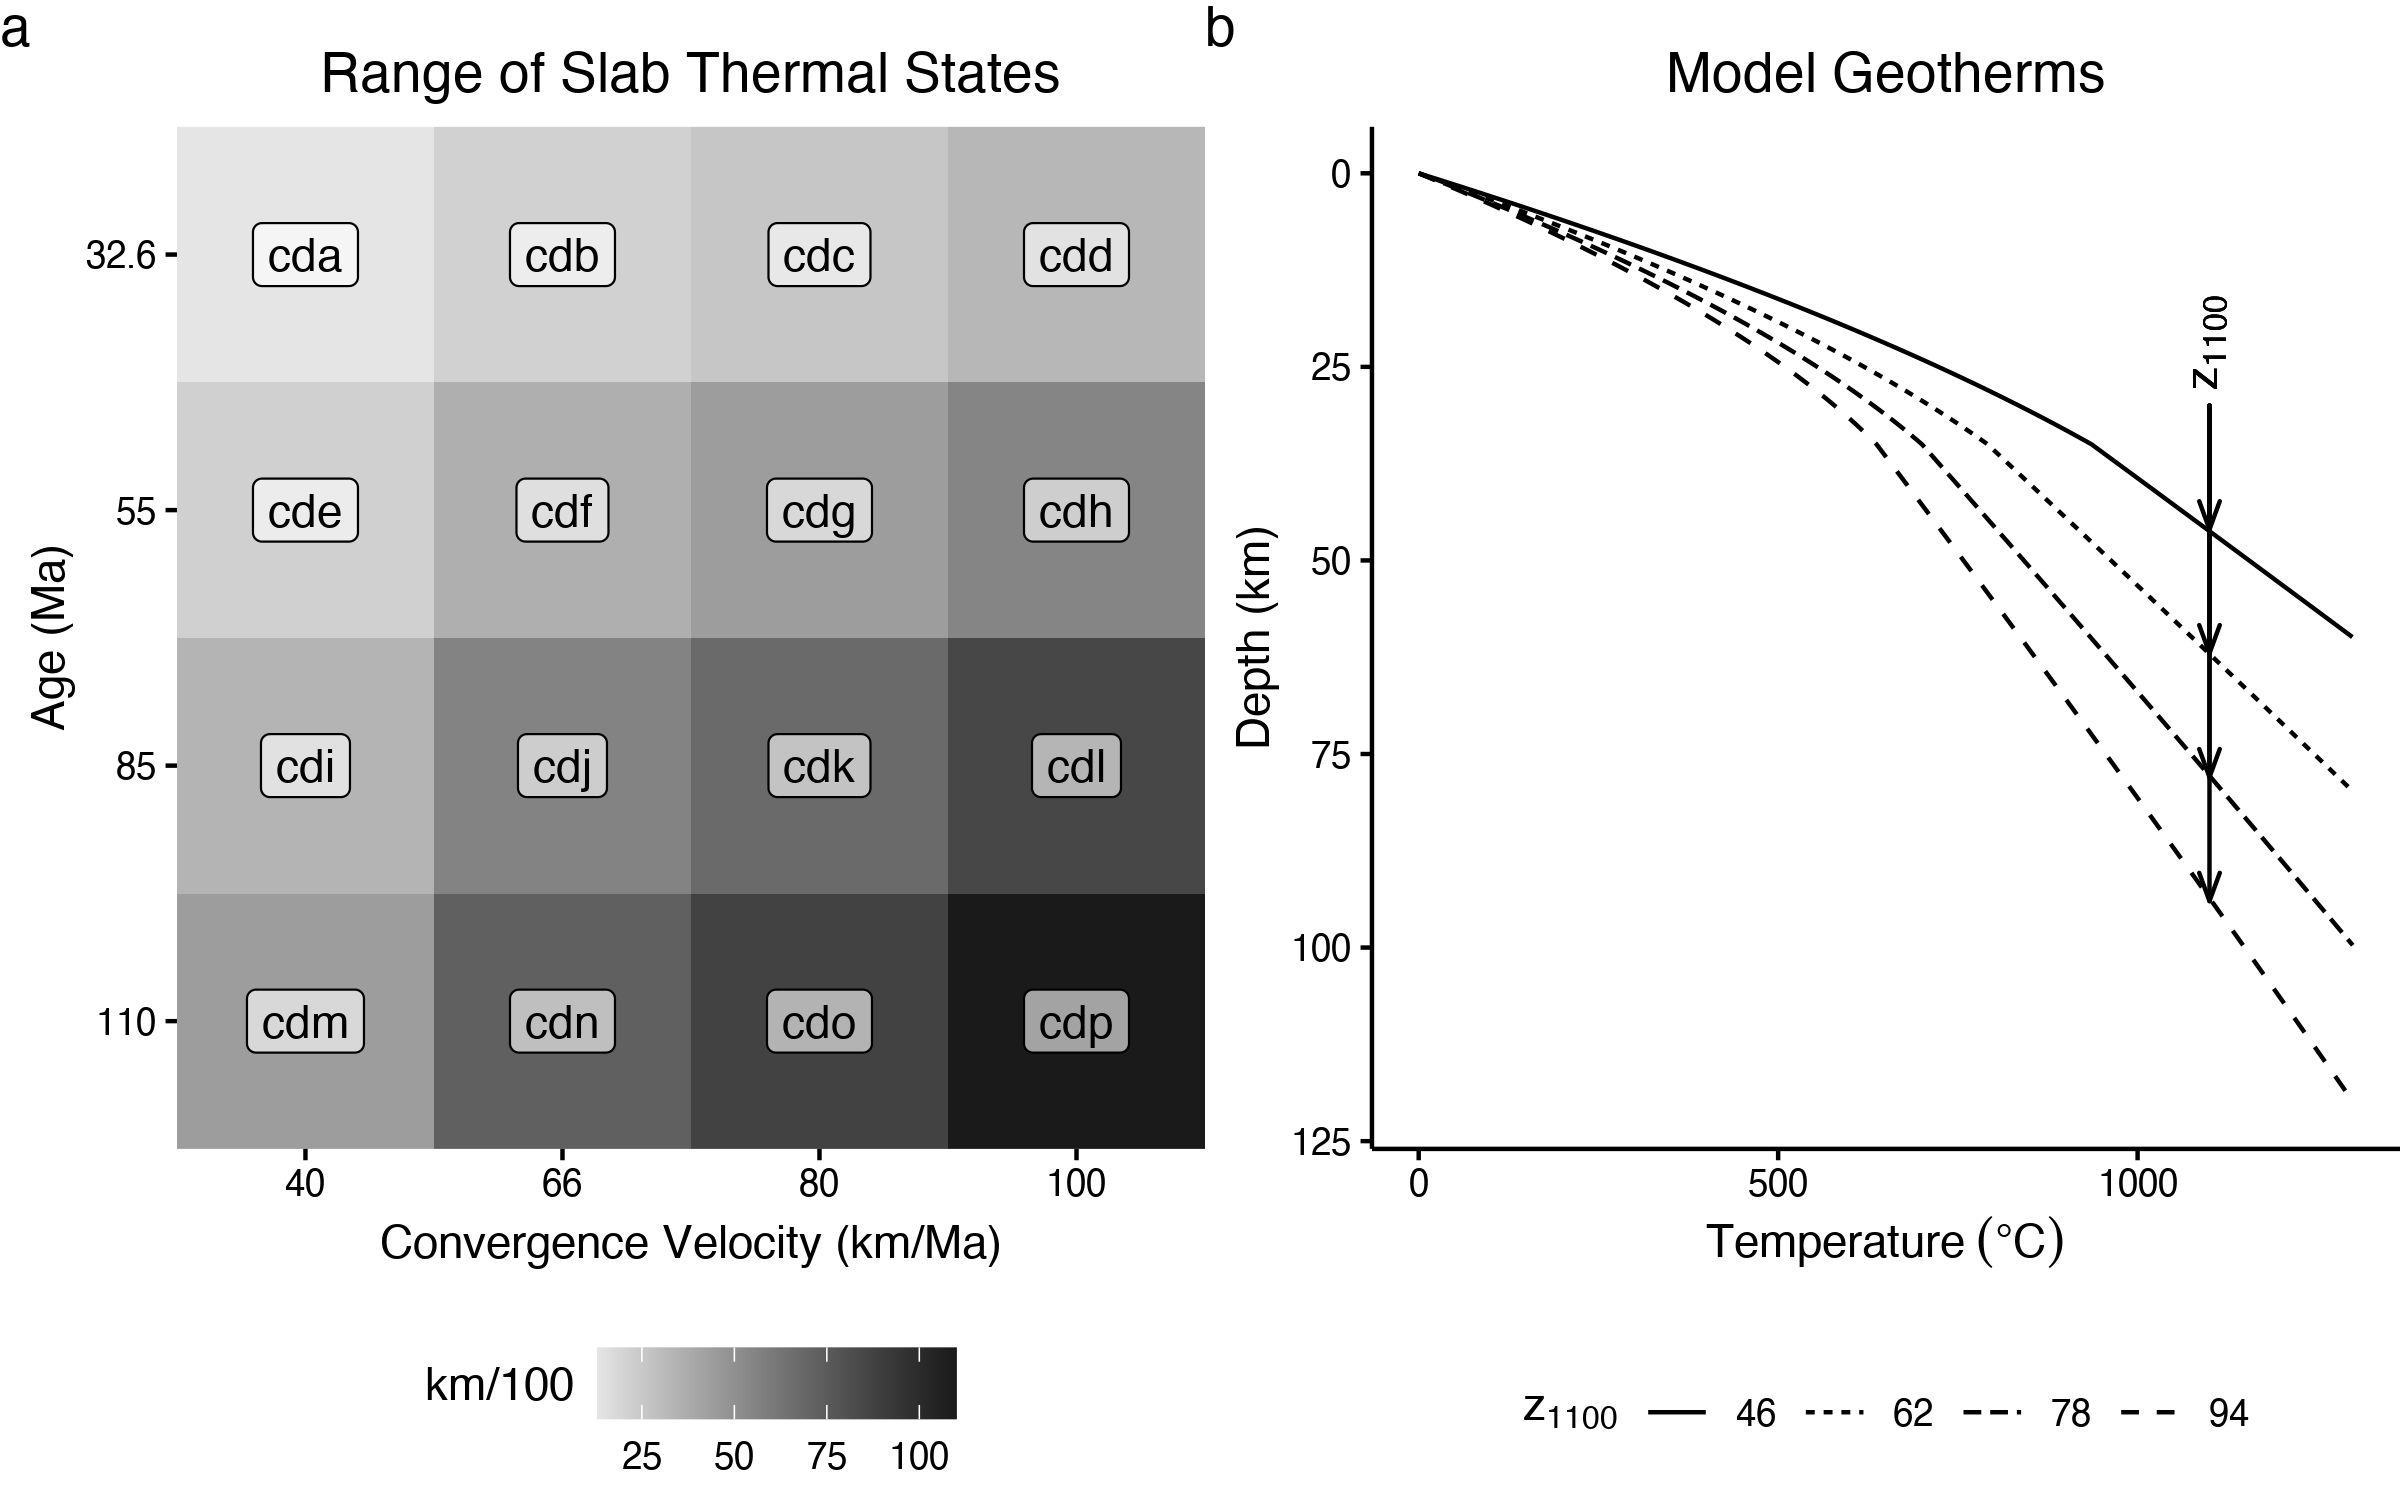
\includegraphics[width=1\linewidth,]{figs/fig2} 

}

\caption{The range of key parameters investigated in this study. (a) Modelled thermal parameters range from 13 to 110 $km/100$ and broadly reflect the distribution of slab ages and convergence velocities in modern subduction zones. Model names include the prefix "cd" for "coupling depth" with increasing alphabetic suffixes. Note that neither axes are continuous. (b) Geotherms were constructed using a one-dimensional steady-state conductive cooling model using $T(z$=$0)$=$0\ ^{\circ}C$ and $q(z$=$0)$=$59,\ 63,\ 69,\ 79\ mW/m^{2}$, and constant radiogenic heating of 1.0 $\mu W/m^{3}$ for a 35 $km$-thick crust and 0.022 $\mu W/m^{3}$ for the mantle. The continental geotherms are calculated up to 1300 $^{\circ}$C, with a 0.5 $^{\circ}C/km$ gradient (the mantle adiabat) for higher temperatures.}\label{fig:params}
\end{figure}

\begin{table}

\caption{\label{tab:melts}Melting curves used in numerical experiments}
\centering
\resizebox{\linewidth}{!}{
\begin{threeparttable}
\begin{tabular}[t]{lrrlrlrrrrr}
\toprule
\multicolumn{1}{c}{} & \multicolumn{8}{c}{Solidus Constants$^1$} & \multicolumn{2}{c}{Liq Constants$^2$} \\
\cmidrule(l{3pt}r{3pt}){2-9} \cmidrule(l{3pt}r{3pt}){10-11}
Material & $a$ & $b$ & $c$ & $d$ & $e$ & $f$ & $g$ & $h$ & $i$ & $j$\\
\midrule
Felsic sediments & 1200 & 889 & 1.79e+04 & 54 & 2.02e+04 & 831 & 0.0600 & 0 & 1262 & 0.009\\
Felsic crust & 1200 & 889 & 1.79e+04 & 54 & 2.02e+04 & 831 & 0.0600 & 0 & 1262 & 0.009\\
Oceanic Crust & 1600 & 973 & 7.04e+05 & 354 & 7.78e+07 & 935 & 0.0035 & 62 & 1423 & 0.105\\
Dry mantle & 0 & 0 & 0 & 0 & 0 & 1394 & 0.1330 & -51 & 2073 & 0.114\\
Hydrated mantle & 2400 & 1240 & 4.98e+04 & 323 & 0 & 0 & 127000.0000 & 35 & 2073 & 0.114\\
\addlinespace
Serpentinized mantle & 2400 & 1240 & 4.98e+04 & 323 & 0 & 0 & 127000.0000 & 35 & 2073 & 0.114\\
\bottomrule
\end{tabular}
\begin{tablenotes}
\item After phase diagrams from Schmidt \& Poli (1998)
\item[1] $T(Solidus)=b+\frac{c}{(P+d)}+\frac{e}{(P+d)^2}$ at $P<a$, $f+gP+hP^2$ at $P\geq a$, $P$ in $[MPa]$, $T$ in $[K]$
\item[2] $T(Liquidus) = i+jP$, $P$ in $[MPa]$, $T$ in $[K]$
\end{tablenotes}
\end{threeparttable}}
\end{table}

\hypertarget{calculating-geotherms-and-defining-lithospheric-thickness}{%
\subsection{Calculating geotherms and defining lithospheric
thickness}\label{calculating-geotherms-and-defining-lithospheric-thickness}}

The oceanic crust was modeled as 1 \(km\) of sediment cover overlying 2
\(km\) of basalt and 5 \(km\) of gabbro (Figure~\ref{fig:init}a).
Oceanic lithosphere was continually made at a pseudo-mid-ocean ridge on
the left boundary of the model (Figure~\ref{fig:init}b) and an enhanced
vertical cooling condition was applied at 200 \(km\) from the mid-ocean
ridge to adjust for the proper oceanic plate age, and therefore its
lithospheric thickness as it enters the trench
(\protect\hyperlink{ref-Agrusta2013}{Agrusta et al., 2013}). We used
plate ages from 32.6 to 110 \(Ma\) and convergence velocities from 40 to
100 \(km/Ma\) (Figure~\ref{fig:params}a). This range of slab parameters
broadly reflects the middle-range of the modern global subduction system
(\protect\hyperlink{ref-Syracuse2006}{Syracuse \& Abers, 2006}).

The initial continental geotherms were determined by solving the heat
flow equation in one-dimension to 1300 \(^{\circ}C\)
(Figure~\ref{fig:params}b). We assumed a fixed temperature of 0
\(^{\circ}C\) at the surface, constant radiogenic heating of 1
\(\mu W/m^{3}\) in the 35 \(km\)-thick continental crust and 0.022
\(\mu W/m^{3}\) in the mantle, and thermal conductivities of 2.3
\(W/mK\) and 3.0 \(W/mK\) for the continental crust and mantle,
respectively. Above, 1300 \(^{\circ}C\), temperature was assumed to
increase by 0.5 \(^{\circ}C/km\) (the mantle adiabat).

Many studies define the base of the continental lithosphere at the 1300
\(^{\circ}C\) isotherm, but it can be determined more accurately from
viscosity and strain rate as the model progresses. The mechanical base
of the lithosphere in our models generally occurred around the 1100
\(^{\circ}C\) isotherm---characterized by a rapid decrease in viscosity
and increase in strain rate
(Figures~\ref{fig:cdfstep1}, \ref{fig:cdfstep2}, \ref{fig:cdfstep3}). As
such, we consider the oceanic and continental lithosphere in this study
as mechanical layers defined by viscosity, rather than merely
temperature. For convenience, we refer to the continental lithospheric
thickness as \(z_{1100}\) because of its general correspondence with the
1100 \(^{\circ}C\) isotherm. Our modelled range of \(z_{1100}\)
corresponds to backarc surface heat flow of 59, 63, 69, and 79
\(mW/m^{2}\).

\hypertarget{metamorphic-dehydration-reactions}{%
\subsection{Metamorphic (de)hydration
reactions}\label{metamorphic-dehydration-reactions}}

Our use of Lagrangian markers to store pressure, temperature, and
rheology allows for subsequent changes of material properties for rocks
undergoing simulated metamorphic reactions. In our models, we focused on
dehydration reactions in the slab and the formation and breakdown of
antigorite in the mantle wedge. For computational efficiency our models
did not solve for thermodynamically stable mineral assemblages to
compute water contents for the slab and mantle wedge (e.g.,
\protect\hyperlink{ref-Connolly2005}{Connolly, 2005}). Instead, we
implemented a simple model for gradual dehydration \DIFdelbegin \DIFdel{(eclogitization ) }\DIFdelend \DIFaddbegin \DIFadd{and eclogitization }\DIFaddend of
oceanic crust\DIFdelbegin \DIFdel{, }\DIFdelend \DIFaddbegin \DIFadd{. Dehydration of oceanic crust is }\DIFaddend computed as a linear
function of depth (lithostatic pressure), with a maximum depth (150
\(km\))\DIFaddbegin \DIFadd{, or temperature (1427 \(^\circ C\)), }\DIFaddend where the slab \DIFdelbegin \DIFdel{was
}\DIFdelend \DIFaddbegin \DIFadd{became
}\DIFaddend completely dehydrated. This approach effectively simulates a continuous
influx of water to the mantle wedge, beginning with compaction and
release of connate water at shallow depths, followed by a sequence of
reactions consuming major hydrous phases (chlorite, lawsonite, zoisite,
chloritoid, talc, amphibole, and phengite) in different parts of the
hydrated basaltic crust (\protect\hyperlink{ref-Schmidt1998}{Schmidt \&
Poli, 1998}; \protect\hyperlink{ref-VanKeken2011}{van Keken et al.,
2011}). \DIFdelbegin \DIFdel{We implicitly assume slabs of different ages release water
similarly. Older slabs, however, should carry water to greater depths
because water-releasing reactions will be delayed along cold subduction
thermal gradients, relative to younger slabs with warmer subduction
thermal gradients }\DIFdelend \DIFaddbegin \DIFadd{Eclogitization was modelled by the garnet-in and plagioclase-out
reactions defined by }\protect\hyperlink{ref-Ito1971}{Ito \& Kennedy}
\DIFaddend (\protect\DIFdelbegin %DIFDELCMD < \hyperlink{ref-Peacock1996}{Peacock, 1996}%%%
\DIFdelend \DIFaddbegin \hyperlink{ref-Ito1971}{1971}\DIFaddend ).

For the mantle wedge, hydration of strong peridotite to form weak
brucite and serpentine along the subduction interface is likely
responsible for mechanical decoupling between the slab and the mantle
wedge at shallow levels (\protect\DIFaddbegin \hyperlink{ref-Agard2016}{Agard et al.,
2016}\DIFadd{; }\protect\DIFaddend \hyperlink{ref-Hyndman2003}{Hyndman \& Peacock, 2003};
\protect\hyperlink{ref-Peacock1999a}{Peacock \& Hyndman, 1999}). If so,
noting that brucite breaks down at much lower temperatures than
serpentine (\protect\hyperlink{ref-Schmidt1998}{Schmidt \& Poli, 1998}),
the loss of serpentine likely represents the key transition from a weak
wedge (and subduction interface) to a strong wedge. Dehydration of
serpentine was modelled as an abrupt, discontinuous reaction, which is a
good approximation for near-endmember compositions, like (Mg-rich)
peridotites. The P-T conditions of the reaction
\(antigorite \Leftrightarrow olivine + orthopyroxene + H_{2}O\) were
based on the experimentally determined stability field from
\protect\hyperlink{ref-Schmidt1998}{Schmidt \& Poli}
(\protect\hyperlink{ref-Schmidt1998}{1998}) and implemented into our
model using the following equation:

\begin{equation}\protect\hypertarget{eq:antstab}{}{\begin{aligned}
  T_{atg-out}(z) &= 751.50+6.008\times10^{-3}z-3.469\times10^{-8}z^2 & & for~z<63000m \\
  T_{atg-out}(z) &= 1013.2-6.039\times10^{-5}z-4.289\times10{-9}z^2 & & for~z>63000m
 \end{aligned}}\label{eq:antstab}\end{equation}

where \(z\) is the depth of a marker from the surface in meters and
\(T\) is temperature in Kelvins. This reaction placement is also
consistent to within 25 \(^{\circ}C\) with recent experiments
(\protect\hyperlink{ref-Shen2015}{Shen et al., 2015}). Under assumptions
of thermodynamic equilibrium, markers whose internal temperature exceeds
\(T(z)\) spontaneously formed \(olivine + orthopyroxene + H_{2}O\),
releasing their crystal-bound water. This implementation is common to
versions of I2VIS that do not implement thermodynamic computations of
mineral stability (e.g., \protect\hyperlink{ref-Connolly2005}{Connolly,
2005}).

\DIFaddbegin \DIFadd{We implicitly assumed slabs of different ages release water similarly.
However, older slabs may carry water to greater depths, relative to
younger slabs, because cold subduction thermal gradients may delay
water-releasing reactions (}\protect\hyperlink{ref-Peacock1996}{Peacock,
1996}\DIFadd{). Stronger slab-age-dependent differences in mechanical coupling
depths were not likely to result by including thermodynamically-computed
water contents in our models because mechanical coupling, as our models
were parameterized, were controlled by the antigorite-out reaction
(Equation~\ref{eq:antstab}). We found that alternate models with abrupt
water release at the antigorite-out reaction stabilized after 5 Ma in a
similar manner to models with gradual water release. The most important
reaction to model was the antigorite-out reaction
(}\protect\hyperlink{ref-Schmidt1998}{Schmidt \& Poli, 1998}\DIFadd{), which was
both pressure- and temperature-dependent (Equation~\ref{eq:antstab}),
and will therefore be affected by differences in slab age. The effects
of explicitly modelling other major dehydration reactions at shallower
depths in the slabs were thus likely to be insignificant and greatly
decrease computational efficiency. We therefore chose a simplified
gradual water release model for all slabs.
}

\DIFaddend The excess water released by a rock marker was modelled as a fluid
particle that migrates through moving rocks with a relative velocity
defined by local \DIFdelbegin \DIFdel{pressure gradients, }\DIFdelend \DIFaddbegin \DIFadd{dynamic (non-lithostatic) pressure gradients (after
}\protect\hyperlink{ref-Faccenda2009}{Faccenda et al., 2009}\DIFadd{). The fluid
velocities are }\DIFaddend scaled by a 10 \(cm/yr\) vertical percolation velocity \DIFdelbegin \DIFdel{corresponding to
a }\DIFdelend \DIFaddbegin \DIFadd{to
account for }\DIFaddend purely lithostatic pressure \DIFdelbegin \DIFdel{gradient }\DIFdelend \DIFaddbegin \DIFadd{gradients }\DIFaddend in the mantle (\DIFaddbegin \DIFadd{after
}\protect\hyperlink{ref-Gorczyk2007}{Gorczyk et al., 2007}\DIFadd{, }\DIFaddend see Appendix,
\DIFdelbegin %DIFDELCMD < \protect\hyperlink{ref-Faccenda2009}{Faccenda et al., 2009}%%%
\DIFdel{)}\DIFdelend \DIFaddbegin \DIFadd{(De-)hydration model)}\DIFaddend . The fluid particle migrates until it reaches
material that can consume an additional amount of water by equilibrium
hydration reactions (e.g., Equation~\ref{eq:antstab}). Theoretically,
the mantle can store large amounts of water because antigorite is stable
at shallow mantle conditions and can contain up to 13 \(wt.\%\) water
(\protect\hyperlink{ref-Reynard2013}{Reynard, 2013}). Thermodynamic
models predict 8 \(wt.\%\) water in the mantle wedge
(\protect\hyperlink{ref-Connolly2005}{Connolly, 2005}). However, seismic
studies suggest that most forearcs are only partially serpentinized
(\(<\) 20-40 \(\%\)), equating to water contents of ca. 3-6 \(wt.\%\)
(\protect\hyperlink{ref-Abers2017}{Abers et al., 2017};
\protect\hyperlink{ref-Carlson2003}{Carlson \& Miller, 2003}). Therefore
we limit mantle wedge hydration to \(\leq\) 2 \(wt.\%\ H_{2}O\) and
assume any \(H_{2}O\) in excess exits the system through channelized
fluid flow (\protect\hyperlink{ref-Davies1999}{Davies, 1999}).

\hypertarget{rheologic-model}{%
\subsection{Rheologic Model}\label{rheologic-model}}

Contributions from dislocation and diffusion creep flow laws are taken
into account by computing a composite rheology for ductile rocks,
\(\eta_{creep}\):

\begin{equation}\protect\hypertarget{eq:ductile}{}{\begin{aligned}\frac{1}{\eta_{creep}} = \frac{1}{\eta_{diff}} + \frac{1}{\eta_{disl}}\end{aligned}}\label{eq:ductile}\end{equation}

\(\eta_{diff}\) and \(\eta_{disl}\) are effective viscosities for
diffusion and dislocation creep, respectively.

For the crust and serpentinized mantle, \(\eta_{diff}\) and
\(\eta_{disl}\) are computed as:

\begin{equation}\protect\hypertarget{eq:crust}{}{\begin{aligned}\eta_{diff} &= \frac{A}{2\sigma_{cr}^{n - 1}}\exp\left( \frac{E + PV}{RT} \right) \\\\
\eta_{disl} &= \frac{1}{2}A^{\frac{1}{n}}\exp\left( \frac{E + PV}{nRT} \right){\dot{\varepsilon}}_{II}^{\frac{1}{n} - 1}\end{aligned}}\label{eq:crust}\end{equation}

where \(R\) is gas constant, \(P\) is pressure, \(T\) is temperature (in
\(K\)),
\({\dot{\varepsilon}}_{II} = \sqrt{1/2{({\dot{\varepsilon}}_{ij})}^{2}}\)
is the square root of the second invariant of the strain rate tensor,
\(\sigma_{cr}\) is the assumed diffusion-dislocation transition stress,
and \(A\), \(E\), \(V\) and \(n\) are the material constant, activation
energy, activation volume, and stress exponent, respectively (Table
\ref{tab:materials}, \protect\hyperlink{ref-Hilairet2007}{Hilairet et
al., 2007}; \protect\hyperlink{ref-Ranalli1995}{Ranalli, 1995}).

For the mantle, \(\eta_{diff}\) and \(\eta_{disl}\) are computed as
(\protect\hyperlink{ref-Karato1993}{Karato \& Wu, 1993}):

\begin{equation}\protect\hypertarget{eq:mantle}{}{\begin{aligned}\eta_{diff} &= \frac{G}{2A_{diff}}\left( \frac{h}{b} \right)^{\frac{m}{n}}\exp\left( \frac{E_{diff} + PV_{diff}}{RT} \right) \\\\
\eta_{disl} &= \frac{G}{2A_{disl}^{\frac{1}{n}}}\exp\left( \frac{E_{disl} + PV_{disl}}{nRT} \right){\dot{\varepsilon}}_{II}^{\frac{1}{n} - 1}\end{aligned}}\label{eq:mantle}\end{equation}

where \(b\)=\(5\times10^{-10}\) \(m\) is Burgers vector,
\(G\)=\(8\times10^{10}\) \(Pa\) is shear modulus, \(h\) is the assumed
grain size, \(m\) is the grain size exponent, and the other flow law
parameters are given in Table \ref{tab:materials}. Our models limited
viscosity for all rocks at \(\eta_{min} = 10^{17}\ Pa \cdot s\) and
\(\eta_{max} = 10^{25}\ Pa \cdot s\).

The ductile rheology, \(\eta_{creep}\), is combined with a brittle
(plastic) rheology to yield an effective viscous-plastic rheology using
the following upper limit for the ductile viscosity:

\begin{equation}\protect\hypertarget{eq:plastic}{}{\begin{aligned}\eta_{creep}\ \  &\leq \frac{C + \mu P}{2{\dot{\varepsilon}}_{II}} \\
\mu\  &= \ \mu_{0} - \gamma\mu_{\gamma} & & for~~\gamma \leq \gamma_0 0 \\
\mu &= \mu_1 & & for~~\gamma > \gamma_0 \\
\gamma &= \int_{}^{}\sqrt{\frac{1}{2}{({\dot{\varepsilon}}_{ij(plastic)})}^{2}}dt\end{aligned}}\label{eq:plastic}\end{equation}

where \(\mu\) is the internal friction coefficient, (\(\mu_0\) and
\(\mu_1\) are the initial and final internal friction coefficients,
respectively, Table \ref{tab:materials}),
\(\mu_\gamma = (\mu_0 - \mu_1)/\gamma_0\) is the fault weakening rate
with integrated plastic strain, \(\gamma\) (\(\gamma_0\)=1 is the upper
strain limit for fracture-related weakening), \(C\) is the rock
compressive strength at \(P\)=0 (Table \ref{tab:materials}), \(t\) is
time (\(s\)), and \({\dot{\varepsilon}}_{ij(plastic)}\) is the plastic
strain rate tensor.

\hypertarget{visualization-and-determination-of-coupling-depth}{%
\subsection{Visualization and determination of coupling
depth}\label{visualization-and-determination-of-coupling-depth}}

For each run (e.g., Figure~\ref{fig:comp}) we made calculations at
\(\sim\) 10 \(Ma\) for surface heat flow (Figure~\ref{fig:comp}a), rock
type (Figure~\ref{fig:comp}b, c), temperature (Figure~\ref{fig:comp}d),
viscosity (Figure~\ref{fig:comp}e), strain rate
(Figure~\ref{fig:comp}f), shear heating (Figure~\ref{fig:comp}g), and
flow velocity (Figure~\ref{fig:comp}h). We chose 10 \(Ma\) because
changes to the overall dynamics and thermal structure are small after
ca. 5 \(Ma\) and the additional 5 \(Ma\) provides sufficient time for
the geodynamics to reach quasi-steady state (see
Figure~\ref{fig:antdepth}).

We determined the mechanical coupling depth, \(z_{c}\), by visualizing
viscosity at \(\sim\) 10 \(Ma\) and selecting a node closest to the
point where the viscosity contrast between the serpentinized- and
non-serpentinized basal mantle wedge diminishes to \(<\) 10\(^{2}\)
\(Pa \cdot s\) (Figure~\ref{fig:comp}e). In this study we assume that
the mechanical coupling depth occurs instantaneously and at a single
node. However, mechanical coupling in reality must be dispersed across a
finite length along the slab-mantle interface. At the resolution of our
models, there was a small area (ca. 5x5 \(km\) or 5x5 nodes) where
\(z_{c}\) could appropriately be determined, giving an uncertainty in
our \(z_{c}\) determination on the order of \(\pm\) 2.5 \(km\).

\begin{figure}[h]

{\centering 
\includegraphics[width=1\linewidth,]{figs/fig3} 

}

\caption{Visualization of model cdf with a 78 $km$-thick backarc lithosphere at $\sim$ 10 $Ma$. (a) Surface heat flow calculated at a depth of 2 $km$ beneath the surface. (b) Rock type for the entire model domain. (c) Rock type in the region from the trench to approximately 220 $km$ into the backarc shows a serpentine layer (pink) lubricating the interface between slab and mantle by 10 $Ma$. Melt is inconspicuous in the arc region because of low melt volumes and quick extraction. The effects of melting are more apparent in viscosity (e) and strain rate (f). (d) Temperature distribution shows strong thermal gradients ("bunching") near the coupling point where serpentine becomes unstable. (e) Log viscosity shows high contrast between the slab and serpentinized mantle in the forearc and low contrast where serpentine becomes unstable. Subvertical structure above coupling point reflects melt migration. (f) Log strain rate shows localized strain in the serpentine layer that expands towards the warm core of the mantle wedge as serpentine becomes unstable. Deformation in the mantle wedge is restricted to beneath the stiff lithosphere and along subvertical melt conduits. (g) Shear heating parallels strain rate and is focused into weakest horizons. (h) Streamlines show focused mantle wedge flow towards the coupling region. Rock type key is given in Table \DIFdelbeginFL \DIFdelFL{3.}\DIFdelendFL \DIFaddbeginFL \DIFaddFL{\ref{tab:rock.type}.}\DIFaddendFL }\label{fig:comp}
\end{figure}

\clearpage

\hypertarget{results}{%
\section{Results}\label{results}}

\hypertarget{coupling-depth-predictors}{%
\subsection{Coupling depth predictors}\label{coupling-depth-predictors}}

Across all 64 numerical models (Figure~\ref{fig:results}, Table
\ref{tab:zc.results}) coupling depth correlates strongly, but not
linearly, with increasing backarc lithospheric thickness
(Figure~\ref{fig:biv}a). This correlation is a key result of our
experiments. Slab thermal parameter alone does not correlate obviously
with coupling depth (Figure~\ref{fig:biv}b). Considering standard least
squares regressions of all possible permutations of the variables
\(z_{1100}\), \(z_{1100}^{2}\), and \(\Phi\), the following equation
optimizes the number of parameters, p value, and \(R^{2}\):

\begin{equation}\protect\hypertarget{eq:zc}{}{\begin{aligned}z_{c} = 4.95 \times 10^{- 3}z_{1100}^{2} - 9.27 \times 10^{- 2}\Phi + 63.6\end{aligned}}\label{eq:zc}\end{equation}

where \(z\) is in \(km\) and \(\Phi\) is in \(km/100\). Regression
results are provided in Tables \ref{tab:anova} and \ref{tab:reg.summary}
and show that alternative linear and quadratic models of \(z_c\)
vs.~\(z_{1100}\) and \(\Phi\) fit the experiments well.
Equation~\ref{eq:zc} permits the prediction of the mechanical coupling
depths in modern subduction zones where \(z_{c}\) can be inverted from
heat flow and \(\Phi\) is estimated.

\begin{figure}[h]

{\centering 
\includegraphics[width=1\linewidth,]{figs/fig4} 

}

\caption{Visual table of coupling depth as determined across a range of lithospheric thicknesses and thermal parameters. Note that the thermal parameter axis is not linear. Corresponding experiments are listed along the top of the array. Coupling depth increases systematically with increasing backarc lithospheric thickness (change in grayscale down columns) for all models. Any trend in coupling depth with respect to slab thermal parameter (change in grayscale across rows) is less apparent.}\label{fig:results}
\end{figure}

\begin{landscape}\begin{table}
\caption{\label{tab:zc.results}Numerical modelling results}

\centering
\fontsize{8}{10}\selectfont
\begin{tabular}[t]{lrrr}
\toprule
Model & $z_{1100}$ & $\Phi$ & $z_c$\\
\midrule
cda46 & 46 & 13.0 & 66\\
cdb46 & 46 & 21.5 & 74\\
cdc46 & 46 & 26.1 & 69\\
cdd46 & 46 & 32.6 & 67\\
cde46 & 46 & 22.0 & 72\\
\addlinespace
cdf46 & 46 & 36.3 & 78\\
cdg46 & 46 & 44.0 & 78\\
cdh46 & 46 & 55.0 & 59\\
cdi46 & 46 & 34.0 & 80\\
cdj46 & 46 & 56.1 & 70\\
\addlinespace
cdk46 & 46 & 68.0 & 58\\
cdl46 & 46 & 85.0 & 65\\
cdm46 & 46 & 44.0 & 79\\
cdn46 & 46 & 72.6 & 70\\
cdo46 & 46 & 88.0 & 68\\
\addlinespace
cdp46 & 46 & 110.0 & 64\\
\bottomrule
\end{tabular}
\centering
\begin{tabular}[t]{lrrr}
\toprule
Model & $z_{1100}$ & $\Phi$ & $z_c$\\
\midrule
cda62 & 62 & 13.0 & 80\\
cdb62 & 62 & 21.5 & 79\\
cdc62 & 62 & 26.1 & 78\\
cdd62 & 62 & 32.6 & 77\\
cde62 & 62 & 22.0 & 87\\
\addlinespace
cdf62 & 62 & 36.3 & 82\\
cdg62 & 62 & 44.0 & 75\\
cdh62 & 62 & 55.0 & 70\\
cdi62 & 62 & 34.0 & 91\\
cdj62 & 62 & 56.1 & 77\\
\addlinespace
cdk62 & 62 & 68.0 & 72\\
cdl62 & 62 & 85.0 & 67\\
cdm62 & 62 & 44.0 & 88\\
cdn62 & 62 & 72.6 & 77\\
cdo62 & 62 & 88.0 & 74\\
\addlinespace
cdp62 & 62 & 110.0 & 75\\
\bottomrule
\end{tabular}
\centering
\begin{tabular}[t]{lrrr}
\toprule
Model & $z_{1100}$ & $\Phi$ & $z_c$\\
\midrule
cda78 & 78 & 13.0 & 87\\
cdb78 & 78 & 21.5 & 94\\
cdc78 & 78 & 26.1 & 97\\
cdd78 & 78 & 32.6 & 97\\
cde78 & 78 & 22.0 & 90\\
\addlinespace
cdf78 & 78 & 36.3 & 90\\
cdg78 & 78 & 44.0 & 88\\
cdh78 & 78 & 55.0 & 85\\
cdi78 & 78 & 34.0 & 97\\
cdj78 & 78 & 56.1 & 91\\
\addlinespace
cdk78 & 78 & 68.0 & 84\\
cdl78 & 78 & 85.0 & 77\\
cdm78 & 78 & 44.0 & 78\\
cdn78 & 78 & 72.6 & 87\\
cdo78 & 78 & 88.0 & 85\\
\addlinespace
cdp78 & 78 & 110.0 & 78\\
\bottomrule
\end{tabular}
\centering
\begin{tabular}[t]{lrrr}
\toprule
Model & $z_{1100}$ & $\Phi$ & $z_c$\\
\midrule
cda94 & 94 & 13.0 & 95\\
cdb94 & 94 & 21.5 & 101\\
cdc94 & 94 & 26.1 & 108\\
cdd94 & 94 & 32.6 & 113\\
cde94 & 94 & 22.0 & 100\\
\addlinespace
cdf94 & 94 & 36.3 & 104\\
cdg94 & 94 & 44.0 & 104\\
cdh94 & 94 & 55.0 & 104\\
cdi94 & 94 & 34.0 & 101\\
cdj94 & 94 & 56.1 & 102\\
\addlinespace
cdk94 & 94 & 68.0 & 101\\
cdl94 & 94 & 85.0 & 107\\
cdm94 & 94 & 44.0 & 106\\
cdn94 & 94 & 72.6 & 102\\
cdo94 & 94 & 88.0 & 98\\
\addlinespace
cdp94 & 94 & 110.0 & 108\\
\bottomrule
\end{tabular}
\end{table}
\end{landscape}

In plots of lithospheric thickness vs.~slab thermal parameter
(Figure~\ref{fig:multiv}a-c), contours of coupling depth are shallowly
sloped, indicating that lithospheric thickness is more important than
slab thermal parameter in predicting coupling depth. Predicted coupling
depth for 17 modern subduction segments where backarc heat flow data are
adequate for inverting for lithospheric thickness (Table \ref{tab:segs},
Figure~\ref{fig:multiv}d) show a wide range of predicted coupling
depths, similar to our model simulations. Predicted coupling depths for
modern subduction zones are distributed quasi-normally, with a mean of
\(\sim\) 82 \(km\) and variation of \(\pm\) 14 \(km\) (2\(\sigma\)
Figure~\ref{fig:multiv}d).

\begin{figure}[h]

{\centering 
\includegraphics[width=1\linewidth,]{figs/fig5} 

}

\caption{Bivariate regressions. (a) Coupling depth vs. lithospheric thickness shows coupling depth increasing nonlinearly with increasing backarc lithospheric thickness, which is best fit by a quadratic curve. The correlation is highly significant (see Tables \ref{tab:anova} and \ref{tab:reg.summary}) and explains more than 80\% of the variance in coupling depth. Lithospheric thickness alone predicts coupling depth well (Tables \ref{tab:anova} and \ref{tab:reg.summary}). (b) Coupling depth vs. slab thermal parameter shows no significant correlation (the slope is not significantly different than zero, Table \ref{tab:reg.summary}). The thermal state of the slab has little effect on coupling depth and cannot be used as a standalone predictor.}\label{fig:biv}
\end{figure}

\begin{table}

\caption{\label{tab:segs}Predicted coupling depth for modern subduction zones}
\centering
\fontsize{8}{10}\selectfont
\begin{tabular}[t]{lrrrrrrr}
\toprule
\multicolumn{1}{c}{Segment} & \multicolumn{1}{c}{$q_s^a$} & \multicolumn{1}{c}{$z_{1100}$} & \multicolumn{1}{c}{$\Phi^b$} & \multicolumn{1}{c}{$z_c^c$} & \multicolumn{1}{c}{$z_c^d$} & \multicolumn{1}{c}{$z_c^e$} & \multicolumn{1}{c}{Ref$^f$} \\
\cmidrule(l{3pt}r{3pt}){1-1} \cmidrule(l{3pt}r{3pt}){2-2} \cmidrule(l{3pt}r{3pt}){3-3} \cmidrule(l{3pt}r{3pt}){4-4} \cmidrule(l{3pt}r{3pt}){5-5} \cmidrule(l{3pt}r{3pt}){6-6} \cmidrule(l{3pt}r{3pt}){7-7} \cmidrule(l{3pt}r{3pt}){8-8}
 & $mWm^{-2}$ & $km$ & $km/100$ & $km$ & $km$ & $km$ & \\
\midrule
N. Cascadia & 75 & 74.2 & 3.4 & 92 & 91 & 90 & 1\\
Nankai & 69 & 96.3 & 6.9 & 107 & 109 & 110 & 1\\
Mexico & 72 & 98.1 & 7.2 & 108 & 111 & 112 & 1\\
Columbia-Ecuador & 80 & 66.4 & 10.4 & 86 & 84 & 84 & 1\\
S.C. Chile & 80 & 66.4 & 20.0 & 85 & 84 & 83 & 1\\
\addlinespace
Kyushu & 69 & 83.2 & 13.5 & 97 & 97 & 96 & 1\\
N. Sumatra & 120 & 26.8 & 25.0 & 57 & 65 & 68 & 2\\
Alaska & 80 & 66.4 & 25.3 & 85 & 83 & 82 & 1\\
N. Chile & 85 & 58.7 & 38.4 & 78 & 77 & 77 & 1\\
N. Costa Rica & 80 & 58.5 & 20.4 & 80 & 79 & 78 & 1\\
\addlinespace
Aleutians & 75 & 51.6 & 39.6 & 73 & 73 & 73 & 1\\
N. Hikurangi & 80 & 58.5 & 41.0 & 78 & 77 & 76 & 1\\
Mariana & 80 & 47.5 & 54.6 & 69 & 70 & 70 & 1\\
Kermadec & 80 & 47.5 & 60.0 & 68 & 69 & 70 & 1\\
Kamchatka & 70 & 80.2 & 77.0 & 89 & 88 & 88 & 1\\
\addlinespace
Izu & 80 & 47.5 & 77.0 & 67 & 68 & 68 & 1\\
NE Japan & 88 & 47.7 & 107.9 & 64 & 65 & 65 & 1\\
\bottomrule
\multicolumn{8}{l}{\rule{0pt}{1em}\textsuperscript{a} Avg. backarc heat flow from Currie \& Hyndman (2006)}\\
\multicolumn{8}{l}{\rule{0pt}{1em}\textsuperscript{b} $\Phi=age \cdot convergence~velocity$; applicable to Equation 4}\\
\multicolumn{8}{l}{\rule{0pt}{1em}\textsuperscript{c} $z_c=z_{1100}+\Phi$}\\
\multicolumn{8}{l}{\rule{0pt}{1em}\textsuperscript{d} $z_c=z_{1100}^2+\Phi$}\\
\multicolumn{8}{l}{\rule{0pt}{1em}\textsuperscript{e} $z_c=z_{1100}+z_{1100}^2+\Phi$}\\
\multicolumn{8}{l}{\rule{0pt}{1em}\textsuperscript{f} 1=Currie \& Hyndman (2006), 2=Wada \& Wang (2009)}\\
\end{tabular}
\end{table}

\begin{figure}[h]

{\centering 
\includegraphics[width=1\linewidth,]{figs/fig6} 

}

\caption{Multivariate regressions and predicted coupling depths for present-day arc segments. Contour plots show predicted coupling depths (contours) as a function of slab thermal parameter and lithospheric thickness for linear (a) and quadratic (b, c) regressions, where (b) is the best fit regression (Equation 6, see Tables \ref{tab:anova} and \ref{tab:reg.summary}). Each black square data point represents a numerical model, and white dots are the predicted coupling depths for modern-day subduction zones (Table \ref{tab:segs}). Coupling depth strongly depends on lithospheric thickness, regardless of the regression. Subduction systems with similar thermal parameters can have quite different predicted coupling depths (e.g., Alaska vs. N. Sumatra), while subduction systems with quite different thermal parameters can have quite similar predicted coupling depths (e.g., Kamchatka vs. N. Cascadia) (d) Distribution of predicted coupling depths for the 17 modern subduction zones shown in (a), (b), and (c). These 17 segments span a large range of thermal parameters but are predicted to have coupling depths of 82 $\pm$ 14 $km$.}\label{fig:multiv}
\end{figure}

\clearpage

\hypertarget{surface-heat-flow}{%
\subsection{Surface heat flow}\label{surface-heat-flow}}

Calculated surface heat flow for numerical models with low to moderate
slab thermal parameters (Figure~\ref{fig:hf}) stabilize at uniform
values in the backarc region, which reflect initial steady-state backarc
geotherms. However, all numerical models show some high-amplitude and
high-frequency positive deviations in heat flow within the arc and
backarc regions (Figure~\ref{fig:hf}), especially for the oldest slabs
with the highest convergence rates (highest \(\Phi\)). These deviations
correspond to strong extensional deformation and heat transport via
lithospheric thinning and melt migration. The effect of fluid and melt
migration is most apparent as subvertical low viscosity, high strain
rate columns above the coupling point (Figure~\ref{fig:comp}e, f). The
backarc is unaffected by fluid and melt migration, making it the best
choice for inverting lithospheric thickness from heat flow. Heat flow
deviations in the arc and backarc regions underscore the importance of
characterizing extensional deformation and local advective heat
transport by fluids before attempting to invert backarc lithospheric
thickness from surface heat flow.

A comparison of surface heat flow across numerical models with identical
slabs, but varying backarc lithospheric thickness (model cdf with 46,
62, 78, and 94 \(km\)-thick lithospheres) shows very similar values of
heat flow in the forearc (normalized distance \(\leq\) 0.75,
Figure~\ref{fig:hf78}). In contrast, surface heat flow in the near-arc
to backarc (normalized distance \(>\) 0.75; Figure~\ref{fig:hf78})
disperses systematically and reflects initial steady-state continental
geotherms (i.e.~lithospheric thickness). In nature, surface heat flow
will depend on fault slip rates and rates of volcanic outputs,
especially in the forearc and arc regions. However, heat flow in the
backarc may remain in steady-state if rates of volcanism and crustal
thinning by extension are low.

\begin{figure}[h]

{\centering 
\includegraphics[width=1\linewidth,]{figs/fig7} 

}

\caption{Surface heat flow vs. normalized distance for numerical models with backarc lithospheric thicknesses of 46, 62, 78, and 94 $km$. Normalized distance is the true distance relative to the trench divided by the distance between the arc and trench. Heat flow is colored according to the slab thermal parameter. High amplitude fluctuations in heat flow in the arc region (normalized distance = 1.0) correspond to vertical migration of fluids and melts. In the backarc region, these fluctuations correspond to backarc extension associated with the oldest and fastest-moving slabs (lighter gray lines). Models with no extension fall within a narrow range of surface heat flow values in the backarc region (darker gray lines).}\label{fig:hf}
\end{figure}

\clearpage

\hypertarget{discussion}{%
\section{Discussion}\label{discussion}}

\hypertarget{reaction-mechanism-and-thermal-controls-on-slab-mantle-mechanical-coupling}{%
\subsection{Reaction Mechanism and Thermal Controls on Slab-Mantle
Mechanical
coupling}\label{reaction-mechanism-and-thermal-controls-on-slab-mantle-mechanical-coupling}}

In our numerical experiments, slab-mantle mechanical coupling is
spatially associated with the reaction of (weak) antigorite to form
(stronger) wet olivine. An antigorite-rich serpentinized subduction
channel spontaneously forms atop the dehydrating slab, localizing
strain, lubricating the slab-mantle interface, and mechanically
decoupling the slab and mantle wedge (e.g.,
\protect\hyperlink{ref-Agard2016}{Agard et al., 2016};
\protect\hyperlink{ref-Ruh2015}{Ruh et al., 2015}). As anticipated, it
is the viscosity increase resulting from the transformation of
antigorite that causes slab-mantle mechanical coupling in our models,
where the depth of this reaction is primarily controlled by a balance of
competing thermal feedbacks acting in the upper plate. Cooling and
hydration of the upper lithospheric mantle wedge (antigorite
stabilization) and heating from the lower circulating asthenospheric
mantle wedge (antigorite destabilization) compete to fix the
antigorite-out reaction at depth (Figure~\ref{fig:arrows}).

\begin{figure}[h]

{\centering 
\includegraphics[width=0.8\linewidth,]{figs/fig8} 

}

\caption{Surface heat flow vs. normalized distance for model cdf with backarc lithospheric thicknesses ranging from 46 to 94 $km$. The range of surface heat flow values in the forearc (normalized distance between 0.0 and 1.0) is narrow and shows little variance until near the arc (normalized distance between 0.75 and 1.0). Surface heat flow broadly disperses in the backarc (normalized distance $>$ 1.0) and reflects the initial continental geotherm (lithospheric thickness). A simple relationship between surface heat flow and lithospheric thickness may be obscured in any region experiencing an addition of heat from extension or vertical migration of fluids, especially within the arc-region.}\label{fig:hf78}
\end{figure}

The entire process can be conceptualized as follows. Cooling of the
mantle wedge occurs mainly via diffusive heat loss to the slab along the
entire length of the subducted slab-top (Figure~\ref{fig:arrows}a). At
shallow levels, water released from the slab stabilizes serpentine in
the overriding mantle, effectively decoupling the slab mechanically from
the mantle (Figure~\ref{fig:arrows}b, point a). This mechanical
decoupling promotes antigorite stabilization to greater depths because
the mantle wedge stagnates and continues to cool and receive water from
the dehydrating slab---a positive feedback for the formation of
serpentinite. Only a thin layer of serpentine forms at the slab-mantle
interface in our models, but it is sufficient to mechanically decouple
the slab and mantle.

At deeper levels, beyond the stability of antigorite, diffusive heat
loss from the mantle to the slab forms a thickening layer of
high-viscosity mantle atop the slab (Figure~\ref{fig:arrows}b, point b).
Downward motion of the slab, plus accreated high-viscosity mantle,
(Figure~\ref{fig:arrows}b, point b) relative to the deepest extent of
the stiff forearc mantle (Figure~\ref{fig:arrows}b, point c) creates a
pressure gradient that attracts flow of the weakest
materials---serpentinite from the up-dip direction
(Figure~\ref{fig:arrows}b, point d)---and hot mantle from below
(Figure~\ref{fig:arrows}b, point e). Flow of hot mantle into the necking
region between points b and c is analogous to passive asthenospheric
upwelling toward a mid-ocean ridge where two strong cooling lithospheric
plates diverge. Highly efficient heat advection from the warm mantle
wedge core (Figure~\ref{fig:arrows}a) prevents formation of
sperentine---thus limiting and stabilizing the coupling depth.

Thermal and petrologic feedbacks---the addition of water into a
diffusively cooling, shallow mantle to produce serpentine vs.~the
advection of heat from the deeper mantle to prevent it---drive coupling
towards steady-state. Our results imply a finely-tuned balance of
serpentine stability can maintain coupling depths in subduction zones
for 10's of Ma.

\hypertarget{the-impact-of-z_1100-and-phi-on-coupling}{%
\subsection{\texorpdfstring{The impact of \(z_{1100}\) and \(\Phi\) on
coupling}{The impact of z\_\{1100\} and \textbackslash Phi on coupling}}\label{the-impact-of-z_1100-and-phi-on-coupling}}

How does backarc lithospheric thickness (\(z_{1100}\)) influence
coupling depth? The lithosphere-asthenosphere boundary of the upper
plate defines the permissible flow field of circulating upper mantle,
limiting highly efficient heat advection to below the base of the
mechanical lithosphere (Figure~\ref{fig:streams}a-d). Thin upper plate
lithospheres (Figure~\ref{fig:streams}a, b) permit shallower mantle
wedge circulation and advection of heat farther up the subduction
interface. This shallow circulation raises the depth of the serpentine
breakdown reaction and mechanical coupling. Thick upper plate
lithospheres (Figure~\ref{fig:streams}c, d) restrict mantle wedge
circulation and advection of heat to deeper levels, shifting the
serpentine breakdown reaction and mechanical coupling to greater depths.

In our models, the thermal state of the slab, as represented by the
thermal parameter (\(\Phi\)), has almost no effect on the mechanical
coupling depth. Previous studies of modern subduction zones also
concluded that coupling appears to be insensitive to slab age and
convergence velocity (\protect\hyperlink{ref-Furukawa1993}{Furukawa,
1993}; \protect\hyperlink{ref-Wada2009}{Wada \& Wang, 2009}). The likely
reason that \(\Phi\) makes so little difference is because slab dynamics
induce a negative feedback between diffusive cooling and advective
heating. High-\(\Phi\) slabs (older slabs with higher velocities) cool
the mantle wedge more effectively, but also result in stronger mantle
circulation and greater heat advection. In contrast, low-\(\Phi\) slabs
(younger slabs with lower velocities) are less effective in cooling the
mantle wedge, but also result in weaker mantle circulation and less heat
advection. That is, the shallow vs.~deep impacts of \(\Phi\) tend to
cancel each other, explaining the lack of strong correlation between
coupling and thermal parameter.

\begin{figure}[h]

{\centering 
\includegraphics[width=1\linewidth,]{figs/fig9} 

}

\caption{Visualization of temperature, viscosity, and velocity near the coupling region at $\sim$ 10 $Ma$ for model cdf with lithospheric thickness of 78 $km$. Velocity arrows are relative to the model boundaries, so the upper mantle wedge has a leftwards velocity equal to the velocity of the upper plate, but is stagnant with respect to itself. (a) High-velocity mantle flow occurs only beneath the lithospheric base (1100$^{\circ}C$), transfering heat towards the coupling region. (b) Log viscosity indicates coupling at the point where the viscosity contrast between the slab and mantle approaches zero. Reference points a-e are used for discussing reaction mechanisms and thermal feedbacks during the transition to slab-mantle mechanical coupling.}\label{fig:arrows}
\end{figure}

\clearpage

\hypertarget{predicting-coupling-depths-in-subduction-zones}{%
\subsection{Predicting Coupling Depths in Subduction
Zones}\label{predicting-coupling-depths-in-subduction-zones}}

Theoretically, coupling depth can be predicted directly from forearc
heat flow using forward modelling techniques to fit surface heat flow
data (e.g., \protect\hyperlink{ref-Wada2009}{Wada \& Wang, 2009}).
However, we caution against using fore-arc heat flow data because a)
forward models adjust the mechanical coupling depth independently from
the backarc thermal structure, which is inconsistent with the inherent
link between mechanical coupling and backarc thermal structure discussed
above (e.g., Figures~\ref{fig:hf78}, \ref{fig:streams}), and b) shear
heating and crustal plutonism can contribute to surface heat flow in the
forearc (\protect\hyperlink{ref-Gao2014}{Gao \& Wang, 2014};
\protect\hyperlink{ref-ReesJones2018}{Rees Jones et al., 2018}),
complicating any simple correspondence with coupling depth.

Instead, we recommend predicting mechanical coupling depth in modern
subduction zones based on Equation~\ref{eq:zc}, estimates of backarc
lithospheric thickness (as estimated from backarc heat flow), and slab
thermal parameter. The slab thermal parameter is inventoried for most
subduction zone segments (\protect\hyperlink{ref-Syracuse2006}{Syracuse
\& Abers, 2006}), but a corresponding dataset of lithospheric
thicknesses does not exist. Several geophysical and petrologic methods
might be considered for independent estimates of lithospheric thickness
(e.g., seismic velocities, flexure, heat flow, mantle xenoliths, etc.),
but we prefer to focus on backarc surface heat flow because of its
correspondence with thermal structure. In this approach, backarc
lithospheric thickness is estimated using simple one-dimensional heat
transport models assuming values for radiogenic heat production in the
crust (e.g., \protect\hyperlink{ref-Rudnick1998}{Rudnick et al., 1998}).
That is, one can use compiled backarc heat flow data to invert for
backarc lithospheric thickness, calculate the slab thermal parameter
from the product of slab age and convergence velocity, and apply
Equation~\ref{eq:zc} to estimate mechanical coupling depth. Of course,
care must be taken to avoid backarcs with strong extensional deformation
or conspicuous heating from magmatism because heat flow in these regions
will underestimate backarc lithospheric thickness and consequently
underestimate coupling depth.

\begin{figure}[h]

{\centering \includegraphics[width=1\linewidth,]{figs/fig10} 

}

\caption{Streamlines for the standard model, cdf, with backarc lithospheric thickness of (a) 46, (b) 62, (c) 78, and (d) 94 $km$. All models are visualized at $\sim$ 10 $Ma$ and plotted on the same scale and location within the model domain. The flow of warm mantle is restricted to below the 1100$^{\circ}C$ isotherm, which corresponds to the base of the backarc lithosphere. A minimum coupling depth appears to exist as models with extremely thin lithospheres (a) exhibit coupling at $\sim$ 70-80 $km$ depth, but increasing $z_{1100}$ increases coupling depth as mantle flow and advective heat transport are diminished.}\label{fig:streams}
\end{figure}

\clearpage

\hypertarget{a-common-coupling-depth-globally}{%
\subsection{A Common Coupling Depth
Globally?}\label{a-common-coupling-depth-globally}}

Mechanical coupling depths in subduction zones are commonly assumed to
fall within a narrow range of 70-80 \(km\)
(\protect\hyperlink{ref-Syracuse2010}{Syracuse et al., 2010};
\protect\hyperlink{ref-Wada2009}{Wada \& Wang, 2009}). We tested the
correlation between backarc lithospheric thickness and coupling depth
using the natural dataset compiled by
\protect\hyperlink{ref-Wada2009}{Wada \& Wang}
(\protect\hyperlink{ref-Wada2009}{2009}) (Figure~\ref{fig:multiv}d).
Much of their dataset is based on
\protect\hyperlink{ref-Currie2006}{Currie \& Hyndman}
(\protect\hyperlink{ref-Currie2006}{2006}), who infer backarc
lithospheric thicknesses for 10 circum-Pacific subduction zones of 50-60
\(km\) (as defined by the 1200 \(^{\circ}C\) isotherm). Backarc
lithospheres are inferred to be relatively thin from uniformly high heat
flow (\(>\) 70 \(mW/m^{2}\)), thermobarometric constraints on mantle
xenoliths, and P-wave velocities
(\protect\hyperlink{ref-Currie2006}{Currie \& Hyndman, 2006}). The mean
value of 82 \(\pm\) 14 \(km\) (2\(\sigma\)) for mechanical coupling
depths in our analysis (Figure~\ref{fig:multiv}d) roughly matches the
preferred depth inferred from forearc heat flow data for Cascadia and NE
Japan (75-80 \(km\), \protect\hyperlink{ref-Syracuse2010}{Syracuse et
al., 2010}; \protect\hyperlink{ref-Wada2009}{Wada \& Wang, 2009})
\(km\), but our predicted coupling depths (Figure~\ref{fig:multiv}d) are
distributed more broadly. For example, omitting Mexico and Nankai
because their \(\Phi\) values fall outside our modeling domain,
predicted coupling depths range from almost 100 \(km\) (Kyushu) to
\(\sim\) 65 \(km\) (Sumatra and NE Japan, Table \ref{tab:segs}).

The petrologic record may also provide insight into the consistency of a
mechanical coupling depth. As it approaches the mechanical coupling
depth, the serpentine channel narrows and focuses return flow. The
demise of the serpentine channel at greater depths may provide a natural
barrier such that rocks within the serpentine channel are more likely to
be exhumed than rocks below the channel. If so, the abundance of
blueschists and eclogites whose maximum burial depths are less than the
pinchout of the serpentine channel, i.e., at the mechanical coupling
depth, should be greater than rocks with greater maximum burial depths.
A cumulative probability distribution of data compiled by
\protect\hyperlink{ref-Penniston2015}{Penniston-Dorland et al.}
(\protect\hyperlink{ref-Penniston2015}{2015}) shows a distinct kink at
an inferred depth of \(\sim\) 80 \(km\) (Figure~\ref{fig:pd15}). Rocks
whose peak metamorphic pressures correspond with depths \(\leq\) 80
\(km\) are much more likely to be exhumed than rocks metamorphosed at
depths \(>\) 80 \(km\). In fact, nearly all examples of rocks exhumed
from greater depths in the compilation of
\protect\hyperlink{ref-Penniston2015}{Penniston-Dorland et al.}
(\protect\hyperlink{ref-Penniston2015}{2015}) were exhumed in the
context of collisions. Logically, the metamorphic record supports a
common mechanical coupling depth of \(\leq\) 80 \(km\).

Relatively high backarc heat flow, especially in circum-Pacific
subduction zones, suggests relatively stable and uniformly thin backarc
lithospheres in mature subduction zones globally that may in turn cause
a common depth of slab-mantle coupling. Although we do not yet fully
understand why the overriding plates may have similar thicknesses, we
can assume that this is likely related to some processes of lithospheric
erosion proposed for subarc lithosphere\DIFdelbegin %DIFDELCMD < {[}%%%
\DIFdel{e. g.,
}%DIFDELCMD < \protect\hyperlink{ref-Arcay2006}{Arcay et al.}
%DIFDELCMD < %%%
\DIFdel{(}%DIFDELCMD < \protect\hyperlink{ref-Arcay2006}{2006}%%%
\DIFdel{); England2010;
}%DIFDELCMD < \protect\hyperlink{ref-Sobolev2005}{Sobolev \& Babeyko}
%DIFDELCMD < %%%
\DIFdel{(}%DIFDELCMD < \protect\hyperlink{ref-Sobolev2005}{2005}%%%
\DIFdel{)}%DIFDELCMD < {]}%%%
\DIFdelend . The following mechanisms of
lithospheric erosion have been proposed: lithospheric delamination
induced by lower crust eclogitization (e.g.,
\protect\hyperlink{ref-Sobolev2005}{Sobolev \& Babeyko, 2005}),
small-scale convection caused by hydration-induced mantle wedge
weakening (e.g., \protect\hyperlink{ref-Arcay2006}{Arcay et al., 2006}),
thermal erosion (e.g., \protect\hyperlink{ref-England2010}{England \&
Katz, 2010}) and mechanical weakening (e.g.,
\protect\hyperlink{ref-Gerya2011}{Gerya \& Meilick, 2011}) by
percolating melts and subarc foundering of magmatic cumulates (e.g.,
\protect\hyperlink{ref-Jull2001}{Jull \& Kelemen, 2001}). Most of these
mechanisms are thus strongly related to mantle wedge hydration, melting,
and melt transport toward volcanic arcs.

\hypertarget{conclusions}{%
\section{Conclusions}\label{conclusions}}

Four important results are highlighted in this study:

\begin{enumerate}
\def\labelenumi{\arabic{enumi}.}
\item
  The antigorite to olivine dehydration reaction stabilizes where
  balance is achieved between competing thermal feedbacks within the
  stagnant mantle wedge lithosphere (diffusive heat loss and inefficient
  heat advection) and circulating mantle wedge asthenosphere (highly
  efficient and focused heat advection). The depth of this reaction, and
  thus mechanical coupling, is primarily dependent on the mechanical
  thickness of the backarc lithosphere.
\item
  A simple expression fitted to the results of our numerical models
  allows the mechanical coupling depth to be calculated for subduction
  zone segments with adequate surface heat flow data in the backarc
  region. Back-arc lithospheric thickness can be inferred from surface
  heat flow using a one-dimensional steady-state conductive cooling
  model. Together with slab thermal parameter , which is tabulated for
  nearly all subduction segments worldwide
  (\protect\hyperlink{ref-Syracuse2010}{Syracuse et al., 2010};
  \protect\hyperlink{ref-Syracuse2006}{Syracuse \& Abers, 2006}),
  coupling depth can be calculated using Equation~\ref{eq:zc}.
\item
  Consistently high backarc heat flow in circum-Pacific subduction zones
  (\protect\hyperlink{ref-Currie2006}{Currie \& Hyndman, 2006};
  \protect\hyperlink{ref-Wada2009}{Wada \& Wang, 2009}) may indicate a
  common depth of slab-mantle mechanical coupling globally at ca. 80
  \(km\). Prior assumptions of slab-mantle mechanical coupling at 70-80
  \(km\) in thermal models are broadly consistent with our results.
\item
  As others have proposed (\protect\hyperlink{ref-Currie2006}{Currie \&
  Hyndman, 2006}; \protect\hyperlink{ref-Wada2009}{Wada \& Wang, 2009})
  subduction zones may self-organize into stable configurations globally
  with warm (thin) upper plate lithospheres and slab-mantle mechanical
  coupling at depths of ca. 80 \(km\). Questions remain, however,
  including: 1) How do warm (thin) backarcs persist over 100's of
  kilometers throughout the lifespan of subduction zones? 2) How abrupt
  is the antigorite-out reaction along the subduction interface?, and 3)
  How can predictive models like Equation~\ref{eq:zc} be improved using
  natural datasets? We propose these questions as topics for future
  research.
\end{enumerate}

\hypertarget{open-research}{%
\section{Open Research}\label{open-research}}

All data, scripts, and instructions for compiling, processing, and
visualizing the data in this study can be found at
\texttt{https://doi.org/10.17605/OSF.IO/ZJAC3}, the official Open
Science Framework data repository. All code is MIT Licensed and freely
for use and distribution (see license details).

\clearpage

\appendix
\section{Appendix}

\hypertarget{subduction-duration-to-achieve-steady-state}{%
\subsection{Subduction duration to achieve steady
state}\label{subduction-duration-to-achieve-steady-state}}

In our models, the stability depth of antigorite along the slab-mantle
interface increases with time as the subducting slab cools and hydrates
the mantle wedge. We observed this process for the first 5 \(Ma\) of
subduction with the antigorite stability depth remaining constant for
ca. 10 \(Ma\) afterwards (Figure~\ref{fig:antdepth}). The change in the
antigorite stability depth, and therefore the slab-mantle mechanical
coupling depth, through ca. 10 \(Ma\) emerges self-consistently in our
models and can help explain how similar configurations, in terms of the
depth to the slab beneath arcs
(\protect\hyperlink{ref-England2004}{England et al., 2004}) and thin
backarc lithospheres (\protect\hyperlink{ref-Currie2006}{Currie \&
Hyndman, 2006}), occur in subduction zones with different slab ages,
convergence rates, geometries, and subduction durations. Our modelling
results indicate that subduction zones quickly (\(<\) 5 \(Ma\)) develop
and stabilize quasi-permanent, generalized configurations with a
slab-mantle mechanical coupling depth dependent on the thickness of the
backarc lithosphere.

Exceptions occur in our models with the thinnest backarc lithospheres
(\(z_{1100}\) = 46 \(km\)), which exhibit transient behavior after ca. 5
\(Ma\) (Figure~\ref{fig:antdepth}). These models rapidly (\(<\) 5
\(Ma\)) develop spreading centers in the backarc because of their
extremely thin (weak) backarc lithospheres. The proximity of a spreading
center in the backarc region diverts heat from the circulating mantle
wedge and interferes with the development of a stable antigorite
breakdown location compared to systems that do not develop a backarc
spreading center. In principle, diversion of heat to the backarc could
lead to cooler subducting slabs (less heat advection) and deeper
coupling. This hypothesis may be tested by artificially increasing the
strength of the backarc lithosphere for models with very thin backarc
lithospheres to prevent high rates of backarc spreading.

\begin{figure}[h]

{\centering 
\includegraphics[width=1\linewidth,]{figs/figA1} 

}

\caption{The depth of antigorite stability at the slab-mantle interface vs. time for models with 46, 62, 78, and 94 $km$-thick backarc lithospheres. Antigorite stabilization deepens for the first ca. 5 $Ma$ of subduction and then remains roughly constant for ca. 10 $Ma$. The exceptions are models with very thin backarc lithospheres, which exhibit transient behavior for at least 15 $Ma$. The final achieved stability depth of antigorite increases with increasing backarc lithospheric thickness.}\label{fig:antdepth}
\end{figure}

\clearpage

\hypertarget{absolute-minimum-coupling-depths}{%
\subsection{Absolute minimum coupling
depths?}\label{absolute-minimum-coupling-depths}}

The form of our preferred quadratic regression model shows shallowing of
coupling depths decelerating with progressively thinner upper plate
lithospheres, reaching a minimum of ca. 60 \(km\). This implies that the
antigorite-out reaction should eventually stabilize at \(\geq\) 60
\(km\) depth even during nascent subduction and in warm systems with
thin upper plate lithospheres. From a theoretical point of view, a thin
upper plate lithosphere could allow high heat transport to the shallow
mantle wedge and hinder stabilization of antigorite altogether. Olivine
plus pyroxene would be the stable mantle minerals, and strong, shallow
coupling between plates would be expected
\protect\hyperlink{ref-Gerya2008}{Gerya et al.}
(\protect\hyperlink{ref-Gerya2008}{2008}). However, our models show that
even the warmest subduction systems eventually stabilize antigorite in
the shallow mantle wedge. This is evident by the increasing depth of
mechanical coupling with time for the first 5 \(Ma\) of subduction
(Figure~\ref{fig:antdepth}).

\begin{figure}[h]

{\centering 
\includegraphics[width=0.8\linewidth,]{figs/figA2} 

}

\caption{Cumulative probability versus peak metamorphic pressures for metamorphic rocks exhumed from subduction zones. The break in slope at ca. 2.5 $GPa$ (ca. 80 $km$) suggests that the relative probability that a rock will exhume from pressures less than ca. 2.5 $GPa$ is substantially greater (steeper slope) than for higher pressure rocks (shallower slope). Nearly all rocks exhumed from pressures greater than ca. 2.5 $GPa$ derive from continental crust and were exhumed during collision. Paucity of data below 0.5 $GPa$ reflects sampling bias because these rocks are at best incipiently metamorphosed and not conducive to thermobarometry.}\label{fig:pd15}
\end{figure}

\begin{table}

\caption{\label{tab:anova}Summary of ANOVA test}
\centering
\fontsize{8}{10}\selectfont
\begin{threeparttable}
\begin{tabular}[t]{llrrrl}
\toprule
\multicolumn{1}{c}{Term} & \multicolumn{1}{c}{Contrast} & \multicolumn{1}{c}{Estimate} & \multicolumn{1}{c}{Upper Bound} & \multicolumn{1}{c}{Lower Bound} & \multicolumn{1}{c}{p value} \\
 &  & $km$ & $km$ & $km$ & \\
\midrule
$z_{1100}$ & 62-46 & 8.3 & 2.5 & 14.0 & 1.84e-03\\
$z_{1100}$ & 78-46 & 18.0 & 12.3 & 23.7 & 1.08e-10\\
$z_{1100}$ & 94-46 & 33.6 & 27.8 & 39.3 & 1.99e-11\\
$z_{1100}$ & 78-62 & 9.8 & 4.0 & 15.5 & 1.83e-04\\
$z_{1100}$ & 94-62 & 25.3 & 19.6 & 31.0 & 1.99e-11\\
\addlinespace
$z_{1100}$ & 94-78 & 15.6 & 9.8 & 21.3 & 7.31e-09\\
\bottomrule
\end{tabular}
\begin{tablenotes}
\item Pair-wise Tukey's test comparing means between groups. Estimates are differences between means. Null hypothesis is that means are not different
\end{tablenotes}
\end{threeparttable}
\end{table}

\begin{table}

\caption{\label{tab:reg.summary}Summary of regression models}
\centering
\fontsize{8}{10}\selectfont
\begin{threeparttable}
\begin{tabular}[t]{llrrl}
\toprule
Model & Term & Estimate & Std. Error & p value\\
\midrule
1 & Intercept & 89.4 & 3.7 & 2.24e-33\\
1 & $\phi$ & -0.1 & 0.1 & 1.55e-01\\
2 & Intercept & 36.4 & 3.2 & 7.15e-17\\
2 & $z_{1100}$ & 0.7 & 0.0 & 3.73e-23\\
3 & Intercept & 58.9 & 1.7 & 1.43e-41\\
\addlinespace
3 & $z_{1100}^2$ & 0.0 & 0.0 & 2.98e-24\\
4 & Intercept & 69.2 & 14.0 & 6.25e-06\\
4 & $z_{1100}$ & -0.3 & 0.4 & 4.63e-01\\
4 & $z_{1100}^2$ & 0.0 & 0.0 & 1.95e-02\\
5 & Intercept & 41.1 & 3.3 & 1.14e-18\\
\addlinespace
5 & $z_{1100}$ & 0.7 & 0.0 & 1.12e-24\\
5 & $\phi$ & -0.1 & 0.0 & 1.18e-03\\
6 & Intercept & 63.6 & 2.1 & 8.29e-39\\
6 & $z_{1100}^2$ & 0.0 & 0.0 & 5.68e-26\\
6 & $\phi$ & -0.1 & 0.0 & 6.98e-04\\
\addlinespace
7 & Intercept & 73.8 & 12.9 & 3.39e-07\\
7 & $z_{1100}$ & -0.3 & 0.4 & 4.23e-01\\
7 & $z_{1100}^2$ & 0.0 & 0.0 & 1.12e-02\\
7 & $\phi$ & -0.1 & 0.0 & 7.28e-04\\
\bottomrule
\end{tabular}
\begin{tablenotes}
\item[1] $z_c=\phi$,
\item[2] $z_c=z_{1100}$
\item[3] $z_c=z_{1100}^2$
\item[4] $z_c=z_{1100}+z_{1100}^2$
\item[5] $z_c=z_{1100}+\phi$
\item[6] $z_c=z_{1100}^2+\phi$
\item[7] $z_c=z_{1100}+z_{1100}^2+\phi$
\end{tablenotes}
\end{threeparttable}
\end{table}

\clearpage

\DIFdelbegin %DIFDELCMD < \hypertarget{de-hydration-model}{%
%DIFDELCMD < \subsection{(De-)hydration model}\label{de-hydration-model}}
%DIFDELCMD < %%%
\DIFdelend \DIFaddbegin \hypertarget{sec:dhydration}{%
\subsection{(De-)hydration model}\label{sec:dhydration}}
\DIFaddend 

The material properties used in our experiments are listed in Tables
\ref{tab:materials} and \ref{tab:melts}. For details about the
sedimentation and erosion, melting and extraction, and rheological
models, please refer to \protect\hyperlink{ref-Sizova2010}{Sizova et
al.} (\protect\hyperlink{ref-Sizova2010}{2010}). Here we discuss only
the hydrodynamic model, because it is the most relevant aspect of our
results.

The hydrodynamics in our models controls the timing and magnitude of
mantle wedge hydration. The main sources of water delivered to the
mantle are altered basaltic crust and seafloor sediments, which we
assumed to contain up to 5 \(wt.\% H_{2}O\). We assumed a gradual
expulsion of water from pore space and through quasi-continuous
dehydration reactions occurring within the slab. Water content is
computed using the following equation:

\[\begin{aligned}\chi_{H_{2}O(wt.\%)} = \chi_{H_{2}O(p_{0})} \times \left( 1 - \frac{\Delta z}{150 \cdot 10^{3}} \right)\end{aligned}\]

where \(\chi_{H_{2}O(p_{0})}\)=5 \(wt.\%\) and \(\Delta z\) is a
marker's depth below the topographical surface.

If a rock marker dehydrates, an independent water particle is
instantaneously generated at the same location with the respective
\(H_{2}O\) content. The new water particle is moved in accordance to the
local velocity field, described by the following equation:

\[\DIFdelbegin %DIFDELCMD < \begin{aligned}
%DIFDELCMD < v_{\text{water}} & = (v_{x},v_{z}) \\
%DIFDELCMD < v_{z} & = v_{z} - v_{z(\text{percolation})} \\
%DIFDELCMD < \end{aligned}%%%
\DIFdelend \DIFaddbegin \begin{aligned}
v_{\text{water}} & = (v_{x(\text{fluid})},v_{z(\text{fluid})}) \\
v_{z(\text{fluid})} & = v_{z(\text{fluid})} - v_{z(\text{percolation})} \\
\end{aligned}\DIFaddend \]

where \(v_{water}\) is the velocity vector of the water particle,
\(v_{x}\) and \(v_{z}\) are the local velocity vectors of the the solid
state mantle or crust, and \(v_{z(percolation)}\) is a prescribed upward
percolation velocity (10 \(cm/year\)). We implicitly neglect kinetics of
reactions, as material properties of markers change instantaneously at
equilibrium reactions.

\hypertarget{approaches-for-implementing-slab-mantle-mechanical-coupling}{%
\subsection{Approaches for implementing slab-mantle mechanical
coupling}\label{approaches-for-implementing-slab-mantle-mechanical-coupling}}

Numerical models employ different approaches to simulate the mechanical
decoupling-coupling transition along the slab-mantle interface. A simple
but highly effective approach is to prescribe a weak layer extending
from the surface to some arbitrary depth or temperature that inhibits
transfer of shear stress across the slab-mantle interface. This approach
is analogous to implementing a no-slip condition and effectively
decouples the slab from the mantle. Numerous models use this method
(e.g., \protect\hyperlink{ref-Peacock1996}{Peacock, 1996};
\protect\hyperlink{ref-Peacock1999b}{Peacock \& Wang, 1999};
\protect\hyperlink{ref-Syracuse2010}{Syracuse et al., 2010};
\protect\hyperlink{ref-Wada2009}{Wada \& Wang, 2009}) in part because it
allows models to be fine-tuned to specific subduction zone
configurations. Serpentine-or talc-rich horizons are typically invoked
to justify mechanical decoupling along the shallow interface.

Our approach does not explicitly define slab-mantle mechanical coupling,
rather we use a rheologic model that explicitly follows experimentally
determined flow laws and mineral stability fields. Conceptually, our
approach follows and extends petrologic explanations for a shallow weak
interface. At lower temperatures, a hydrated, serpentine-rich, or
possibly talc-rich, layer mechanically decouples the mantle wedge from
the subducting slab (\protect\hyperlink{ref-Hyndman2003}{Hyndman \&
Peacock, 2003}; \protect\hyperlink{ref-Peacock1999a}{Peacock \& Hyndman,
1999}). If so, as a corollary, dehydration of serpentine, or possibly
talc, at high temperatures must strengthen the interface. In that
context, and noting that talc is unstable at P \(>\) 2.0 \(GPa\) in an
ultramafic rock (\protect\hyperlink{ref-Schmidt1998}{Schmidt \& Poli,
1998}) \(>\) \(GPa\) , we assigned a serpentine rheology for P-T
conditions below the serpentine-out reaction, and a wet peridotite
rheology above it.

To test the sensitivity of coupling on our rheologic model, we ran
diverse experiments that adjusted the rheology of antigorite, the shape
and position of the antigorite-out reaction, and certain hydrodynamic
parameters. For brevity, these results are not presented here. The
experiments included: 1) antigorite = wet olivine flow law, 2)
antigorite and wet olivine = dry olivine flow law, 3) isothermal
antigorite reaction (straight, vertical reaction line) at 690
\(^{\circ}C\), 4) antigorite reaction with positive nonlinear Clapeyron
slope until 715 \(^{\circ}C\), where it changes to isothermal (kinked
reaction line), 5) linear antigorite reaction with positive Clapeyron
slope (straight, sloped reaction line), 6) linear release of
antigorite-bound \(H_{2}O\) with depth (instead of abrupt release at
equilibrium dehydration reaction), and 7) no fluid-induced weakening
(pore-pressure = 0).

Only experiments 5 and 7 listed above were inconsistent with the results
presented in the present study. Experiment 5 resulted in transient
coupling depths and disjointed antigorite stability in the mantle wedge,
whereas experiment 7 resulted in two-sided subduction (e.g.,
\protect\hyperlink{ref-Gerya2008}{Gerya et al., 2008}). These
experiments suggest that the coupling mechanism in our models is mostly
contingent on the availability of fluids to the mantle wedge and the
shape of the equilibrium antigorite reaction, and relatively insensitive
to the exact flow law parameters.

\begin{figure}[h]

{\centering 
\includegraphics[width=1\linewidth,]{figs/figA3} 

}

\caption{Visualizations of standard model cdf78 at 1.64 Ma. (a) Rock type. (b) Temperature. (c) Log$_{10}$ of viscosity. (d) Streamlines. Early subduction is facilitated by the prescribed initial weak layer cutting the lithosphere. Strain is localized in the weak serpentine layer at the slab-mantle interface. The mantle wedge is stagnant and loses heat to the slab, which promotes antigorite stabiliization to greater depths. Rock type colors are given in Table \ref{tab:rock.type}.}\label{fig:cdfstep1}
\end{figure}

\begin{figure}[h]

{\centering 
\includegraphics[width=1\linewidth,]{figs/figA4} 

}

\caption{Visualization s of standard model cdf78 at 5.05 $Ma$. (a) Rock type. (b) Temperature. (c) Log$_{10}$ of viscosity. (d) Streamlines. By 5 $Ma,$ balance is achieved between heat sinking from the upper mantle wedge to lower parts of the mantle and strong advection of heat in the circulating part of the mantle wedge. A feedback has already developed---heat advection inhibits antigorite stabilization to greater depths. Rock type colors are given in Table \ref{tab:rock.type}.}\label{fig:cdfstep2}
\end{figure}

\begin{figure}[h]

{\centering 
\includegraphics[width=1\linewidth,]{figs/figA5} 

}

\caption{Visualization s of standard model cdf78 at 9.93 $Ma$. (a) Rock type. (b) Temperature. (c) Log$_{10}$ of viscosity. (d) Streamlines. The geodynamics and thermal structure remain approximately constant from 5 $Ma$ (cf. Figure A.4). The system remains in steady state for as long as enough water is supplied to the upper mantle wedge to stabilize antigorite.Rock type colors are given in Table \ref{tab:rock.type}.}\label{fig:cdfstep3}
\end{figure}

\clearpage

\acknowledgments

We thank the Geophysical Fluid Dynamics group at the Institut für
Geophysik, ETH Zürich, for their computing resources and invaluable
instruction, discussion, and support on the numerical modelling methods.
We also thank P. Agard, L. Le Pourhiet, and their students at ISTeP,
Sorbonne Université, for suggestions on the numerical modelling methods
and discussions that greatly enhanced this study. We thank the anonymous
reviewers for their helpful comments and suggestions, which greatly
improved the manuscript. This work was supported by the National Science
Foundation grant OIA1545903 to M. Kohn, S. Penniston-Dorland, and M.
Feineman. Datasets and tools for reproducing the research in this study
are available at (\texttt{https://doi.org/10.17605/OSF.IO/ZJAC3})

\newpage

\hypertarget{references}{%
\section*{References}\label{references}}
\addcontentsline{toc}{section}{References}

\hypertarget{refs}{}
\begin{CSLReferences}{1}{0}
\leavevmode\vadjust pre{\hypertarget{ref-Abers2017}{}}%
Abers, G. A., van Keken, P. E., \& Hacker, B. R. (2017). {The cold and
relatively dry nature of mantle forearcs in subduction zones}.
\emph{Nature Geoscience}, \emph{10}(5), 333--337.

\leavevmode\vadjust pre{\hypertarget{ref-Agard2009}{}}%
Agard, P., Yamato, P., Jolivet, L., \& Burov, E. (2009). {Exhumation of
oceanic blueschists and eclogites in subduction zones: Timing and
mechanisms}. \emph{Earth-Science Reviews}, \emph{92}(1-2), 53--79.

\leavevmode\vadjust pre{\hypertarget{ref-Agard2016}{}}%
Agard, P., Yamato, P., Soret, M., Prigent, C., Guillot, S., Plunder, A.,
et al. (2016). {Plate interface rheological switches during subduction
infancy: Control on slab penetration and metamorphic sole formation}.
\emph{Earth and Planetary Science Letters}, \emph{451}, 208--220.

\leavevmode\vadjust pre{\hypertarget{ref-Agrusta2013}{}}%
Agrusta, R., Arcay, D., Tommasi, A., Davaille, A., Ribe, N., \& Gerya,
T. (2013). {Small-scale convection in a plume-fed low-viscosity layer
beneath a moving plate}. \emph{Geophysical Journal International},
\emph{194}(2), 591--610.

\leavevmode\vadjust pre{\hypertarget{ref-Arcay2006}{}}%
Arcay, D., Doin, M. P., Tric, E., Bousquet, R., \& Capitani, C. de.
(2006). Overriding plate thinning in subduction zones: Localized
convection induced by slab dehydration. \emph{Geochemistry, Geophysics,
Geosystems}, \emph{7}(2).

\leavevmode\vadjust pre{\hypertarget{ref-Burg2005}{}}%
Burg, J. P., \& Gerya, T. (2005). The role of viscous heating in
barrovian metamorphism of collisional orogens: Thermomechanical models
and application to the lepontine dome in the central alps. \emph{Journal
of Metamorphic Geology}, \emph{23}(2), 75--95.

\leavevmode\vadjust pre{\hypertarget{ref-Carlson2003}{}}%
Carlson, R. L., \& Miller, D. J. (2003). Mantle wedge water contents
estimated from seismic velocities in partially serpentinized
peridotites. \emph{Geophysical Research Letters}, \emph{30}(5).

\leavevmode\vadjust pre{\hypertarget{ref-Connolly2005}{}}%
Connolly, J. A. D. (2005). {Computation of phase equilibria by linear
programming: A tool for geodynamic modeling and its application to
subduction zone decarbonation}. \emph{Earth and Planetary Science
Letters}, \emph{236}(1-2), 524--541.

\leavevmode\vadjust pre{\hypertarget{ref-Currie2006}{}}%
Currie, C. A., \& Hyndman, R. D. (2006). {The thermal structure of
subduction zone back arcs}. \emph{Journal of Geophysical Research},
\emph{111}(August), 1--22.

\leavevmode\vadjust pre{\hypertarget{ref-Currie2004}{}}%
Currie, C. A., Wang, K., Hyndman, R. D., \& He, J. (2004). {The thermal
effects of steady-state slab-driven mantle flow above a subducting
plate: The Cascadia subduction zone and backarc}. \emph{Earth and
Planetary Science Letters}, \emph{223}(1-2), 35--48.

\leavevmode\vadjust pre{\hypertarget{ref-Cizkova2013}{}}%
Čížková, H., \& Bina, C. R. (2013). {Effects of mantle and
subduction-interface rheologies on slab stagnation and trench rollback}.
\emph{Earth and Planetary Science Letters}, \emph{379}, 95--103.

\leavevmode\vadjust pre{\hypertarget{ref-Davies1999}{}}%
Davies, J. H. (1999). {The role of hydraulic fractures and intermediate
depth earthquakes in generating suduction zone magmatism}.
\emph{Nature}, \emph{417}(March), 142--145.

\leavevmode\vadjust pre{\hypertarget{ref-England2010}{}}%
England, P., \& Katz, R. F. (2010). Melting above the anhydrous solidus
controls the location of volcanic arcs. \emph{Nature}, \emph{467}(7316),
700--703.

\leavevmode\vadjust pre{\hypertarget{ref-England2004}{}}%
England, P., Engdahl, R., \& Thatcher, W. (2004). {Systematic variation
in the depths of slabs beneath arc volcanoes}. \emph{Geophysical Journal
International}, \emph{156}(2), 377--408.

\leavevmode\vadjust pre{\hypertarget{ref-Faccenda2009}{}}%
Faccenda, M., Gerya, T., \& Burlini, L. (2009). {Deep slab hydration
induced by bending-related variations in tectonic pressure}.
\emph{Nature Geoscience}, \emph{2}(11), 790--793.

\leavevmode\vadjust pre{\hypertarget{ref-Furukawa1993}{}}%
Furukawa, Y. (1993). {Magmatic Processes Under Arcs and Formation of the
Volcanic Front}. \emph{Journal of Geophysical Research}, \emph{98},
8309--8319.

\leavevmode\vadjust pre{\hypertarget{ref-Gao2014}{}}%
Gao, X., \& Wang, K. (2014). {Strength of stick-slip and creeping
subduction megathrusts from heat flow observations}. \emph{Science},
\emph{345}(6200), 1038--1041.

\leavevmode\vadjust pre{\hypertarget{ref-Gao2017}{}}%
Gao, X., \& Wang, K. (2017). {Rheological separation of the megathrust
seismogenic zone and episodic tremor and slip}. \emph{Nature},
\emph{543}(7645), 416--419.

\leavevmode\vadjust pre{\hypertarget{ref-Gerya2011}{}}%
Gerya, T., \& Meilick, F. I. (2011). Geodynamic regimes of subduction
under an active margin: Effects of rheological weakening by fluids and
melts. \emph{Journal of Metamorphic Geology}, \emph{29}(1), 7--31.

\leavevmode\vadjust pre{\hypertarget{ref-Gerya2003}{}}%
Gerya, T., \& Yuen, D. A. (2003). {Characteristics-based marker-in-cell
method with conservative finite-differences schemes for modeling
geological flows with strongly variable transport properties}.
\emph{Physics of the Earth and Planetary Interiors}, \emph{140}(4),
293--318.

\leavevmode\vadjust pre{\hypertarget{ref-Gerya2008}{}}%
Gerya, T., Connolly, J. A. D., \& Yuen, D. A. (2008). {Why is
terrestrial subduction one-sided?} \emph{Geology}, \emph{36}(1), 43--46.

\leavevmode\vadjust pre{\DIFaddbegin \hypertarget{ref-Gonzalez2016}{}}%DIF > 
\DIFadd{Gonzalez, C. M., Gorczyk, W., \& Gerya, T. (2016). Decarbonation of
subducting slabs: Insight from petrological--thermomechanical modeling.
}\emph{\DIFadd{Gondwana Research}}\DIFadd{, }\emph{\DIFadd{36}}\DIFadd{, 314--332.
}

\leavevmode\vadjust \DIFadd{pre}{\DIFaddend \hypertarget{ref-Gorczyk2007}{}}%
Gorczyk, W., Willner, A. P., Gerya, T., Connolly, J. A. D., \& Burg, J.
P. (2007). {Physical controls of magmatic productivity at Pacific-type
convergent margins: Numerical modelling}. \emph{Physics of the Earth and
Planetary Interiors}, \emph{163}(1-4), 209--232.

\leavevmode\vadjust pre{\hypertarget{ref-Grove2012}{}}%
Grove, T. L., Till, C. B., \& Krawczynski, M. J. (2012). {The Role of H
2 O in Subduction Zone Magmatism}. \emph{Annual Review of Earth and
Planetary Sciences}, \emph{40}(1), 413--439.

\leavevmode\vadjust pre{\hypertarget{ref-Hacker2003}{}}%
Hacker, B. R., Peacock, S. M., Abers, G. A., \& Holloway, S. D. (2003).
{Subduction factory 2. Are intermediate-depth earthquakes in subducting
slabs linked to metamorphic dehydration reactions?} \emph{Journal of
Geophysical Research: Solid Earth}, \emph{108}(B1).

\leavevmode\vadjust pre{\hypertarget{ref-Hilairet2007}{}}%
Hilairet, N., Reynard, B., Wang, Y., Daniel, I., Merkel, S., Nishiyama,
N., \& Petitgirard, S. (2007). High-pressure creep of serpentine,
interseismic deformation, and initiation of subduction. \emph{Science},
\emph{318}(5858), 1910--1913.

\leavevmode\vadjust pre{\hypertarget{ref-Hyndman2003}{}}%
Hyndman, R. D., \& Peacock, S. M. (2003). Serpentinization of the
forearc mantle. \emph{Earth and Planetary Science Letters},
\emph{212}(3-4), 417--432.

\leavevmode\vadjust pre{\DIFaddbegin \hypertarget{ref-Ito1971}{}}%DIF > 
\DIFadd{Ito, K., \& Kennedy, G. C. (1971). An experimental study of the
basalt-garnet granulite-eclogite transition. }\emph{\DIFadd{The Structure and
Physical Properties of the Earth's Crust}}\DIFadd{, }\emph{\DIFadd{14}}\DIFadd{, 303--314.
}

\leavevmode\vadjust \DIFadd{pre}{\DIFaddend \hypertarget{ref-Jull2001}{}}%
Jull, M., \& Kelemen, P. B. (2001). On the conditions for lower crustal
convective instability. \emph{Journal of Geophysical Research: Solid
Earth}, \emph{106}(B4), 6423--6446.

\leavevmode\vadjust pre{\hypertarget{ref-Karato1993}{}}%
Karato, S., \& Wu, P. (1993). Rheology of the upper mantle: A synthesis.
\emph{Science}, \emph{260}(5109), 771--778.

\leavevmode\vadjust pre{\hypertarget{ref-McKenzie1969}{}}%
McKenzie, D. P. (1969). {Speculations on the Consequences and Causes of
Plate Motions}. \emph{Geophysical Journal International}, \emph{18}(1),
1--32.

\leavevmode\vadjust pre{\hypertarget{ref-Peacock1990}{}}%
Peacock, S. M. (1990). Fluid processes in subduction zones.
\emph{Science}, \emph{248}(4953), 329--337.

\leavevmode\vadjust pre{\hypertarget{ref-Peacock1991}{}}%
Peacock, S. M. (1991). Numerical simulation of subduction zone
pressure-temperature-time paths: Constraints on fluid production and arc
magmatism. \emph{Philosophical Transactions of the Royal Society of
London. Series A: Physical and Engineering Sciences}, \emph{335}(1638),
341--353.

\leavevmode\vadjust pre{\hypertarget{ref-Peacock1993}{}}%
Peacock, S. M. (1993). The importance of blueschist \(\rightarrow\)
eclogite dehydration reactions in subducting oceanic crust.
\emph{Geological Society of America Bulletin}, \emph{105}(5), 684--694.

\leavevmode\vadjust pre{\hypertarget{ref-Peacock1996}{}}%
Peacock, S. M. (1996). Thermal and petrologic structure of subduction
zones. \emph{Subduction: Top to Bottom}, \emph{96}, 119--133.

\leavevmode\vadjust pre{\hypertarget{ref-Peacock1999a}{}}%
Peacock, S. M., \& Hyndman, R. D. (1999). {Hydrous minerals in the
mantle wedge and the maximum depth of subduction thrust earthquakes}.
\emph{Geophysical Research Letters}, \emph{26}(No. 16), 2517--2520.

\leavevmode\vadjust pre{\hypertarget{ref-Peacock1999b}{}}%
Peacock, S. M., \& Wang, K. (1999). Seismic consequences of warm versus
cool subduction metamorphism: Examples from southwest and northeast
japan. \emph{Science}, \emph{286}(5441), 937--939.

\leavevmode\vadjust pre{\hypertarget{ref-Peacock1994}{}}%
Peacock, S. M., Rushmer, T., \& Thompson, A. B. (1994). Partial melting
of subducting oceanic crust. \emph{Earth and Planetary Science Letters},
\emph{121}(1-2), 227--244.

\leavevmode\vadjust pre{\hypertarget{ref-Penniston2015}{}}%
Penniston-Dorland, S. C., Kohn, M. J., \& Manning, C. E. (2015). The
global range of subduction zone thermal structures from exhumed
blueschists and eclogites: Rocks are hotter than models. \emph{Earth and
Planetary Science Letters}, \emph{428}, 243--254.

\leavevmode\vadjust pre{\hypertarget{ref-Ranalli1995}{}}%
Ranalli, G. (1995). \emph{Rheology of the earth}. Springer Science \&
Business Media.

\leavevmode\vadjust pre{\hypertarget{ref-ReesJones2018}{}}%
Rees Jones, D. W., Katz, R. F., Tian, M., \& Rudge, J. F. (2018).
{Thermal impact of magmatism in subduction zones}. \emph{Earth and
Planetary Science Letters}, \emph{481}, 73--79.

\leavevmode\vadjust pre{\hypertarget{ref-Reynard2013}{}}%
Reynard, B. (2013). {Serpentine in active subduction zones}.
\emph{Lithos}, \emph{178}, 171--185.

\leavevmode\vadjust pre{\hypertarget{ref-Rudnick1998}{}}%
Rudnick, R. L., McDonough, W. F., \& O\&apos;Connell, R. J. (1998).
{Thermal structure, thickness and composition of continental
lithosphere}. \emph{Chemical Geology}, \emph{145}(3-4), 395--411.

\leavevmode\vadjust pre{\hypertarget{ref-Ruh2015}{}}%
Ruh, J. B., Le Pourhiet, L., Agard, P., Burov, E., \& Gerya, T. (2015).
{Tectonic slicing of subducting oceanic crust along plate interfaces:
Numerical modeling}. \emph{Geochemistry, Geophysics, Geosystems},
\emph{16}(10), 3505--3531.

\leavevmode\vadjust pre{\hypertarget{ref-Schmidt1998}{}}%
Schmidt, M. W., \& Poli, S. (1998). {Experimentally based water budgets
for dehydrating slabs and consequences for arc magma generation}.
\emph{Earth and Planetary Science Letters}, \emph{163}(1-4), 361--379.

\leavevmode\vadjust pre{\hypertarget{ref-Shen2015}{}}%
Shen, T., Hermann, J., Zhang, L., Lü, Z., Padrón-Navarta, J. A., Xia,
B., \& Bader, T. (2015). UHP metamorphism documented in
ti-chondrodite-and ti-clinohumite-bearing serpentinized ultramafic rocks
from chinese southwestern tianshan. \emph{Journal of Petrology},
\emph{56}(7), 1425--1458.

\leavevmode\vadjust pre{\hypertarget{ref-Sizova2010}{}}%
Sizova, E., Gerya, T., Brown, M., \& Perchuk, L. L. (2010). {Subduction
styles in the Precambrian: Insight from numerical experiments}.
\emph{Lithos}, \emph{116}(3-4), 209--229.

\leavevmode\vadjust pre{\hypertarget{ref-Sobolev2005}{}}%
Sobolev, S. V., \& Babeyko, A. Y. (2005). What drives orogeny in the
andes? \emph{Geology}, \emph{33}(8), 617--620.

\leavevmode\vadjust pre{\hypertarget{ref-Syracuse2006}{}}%
Syracuse, E. M., \& Abers, G. A. (2006). {Global compilation of
variations in slab depth beneath arc volcanoes and implications}.
\emph{Geochemistry, Geophysics, Geosystems}, \emph{7}(5).

\leavevmode\vadjust pre{\hypertarget{ref-Syracuse2010}{}}%
Syracuse, E. M., van Keken, P. E., Abers, G. A., Suetsugu, D., Bina, C.
R., Inoue, T., et al. (2010). {The global range of subduction zone
thermal models}. \emph{Physics of the Earth and Planetary Interiors},
\emph{183}(1-2), 73--90.

\leavevmode\vadjust pre{\hypertarget{ref-VanKeken2011}{}}%
van Keken, P. E., Hacker, B. R., Syracuse, E. M., \& Abers, G. A.
(2011). {Subduction factory: 4. Depth-dependent flux of H 2 O from
subducting slabs worldwide}. \emph{Journal of Geophysical Research},
\emph{116}(B1), B01401.

\leavevmode\vadjust pre{\hypertarget{ref-VanKeken2018}{}}%
van Keken, P. E., Wada, I., Abers, G. A., Hacker, B. R., \& Wang, K.
(2018). {Mafic High-Pressure Rocks Are Preferentially Exhumed From Warm
Subduction Settings}. \emph{Geochemistry, Geophysics, Geosystems},
\emph{19}(9), 2934--2961.

\leavevmode\vadjust pre{\hypertarget{ref-Wada2009}{}}%
Wada, I., \& Wang, K. (2009). {Common depth of slab-mantle decoupling:
Reconciling diversity and uniformity of subduction zones}.
\emph{Geochemistry, Geophysics, Geosystems}, \emph{10}(10), n/a--n/a.

\leavevmode\vadjust pre{\hypertarget{ref-Wada2008}{}}%
Wada, I., Wang, K., He, J., \& Hyndman, R. D. (2008). {Weakening of the
subduction interface and its effects on surface heat flow, slab
dehydration, and mantle wedge serpentinization}. \emph{Journal of
Geophysical Research: Solid Earth}, \emph{113}(4), 1--15.

\leavevmode\vadjust pre{\hypertarget{ref-Wada2012}{}}%
Wada, I., Behn, M. D., \& Shaw, A. M. (2012). {Effects of heterogeneous
hydration in the incoming plate, slab rehydration, and mantle wedge
hydration on slab-derived H 2O flux in subduction zones}. \emph{Earth
and Planetary Science Letters}, \emph{353-354}, 60--71.

\leavevmode\vadjust pre{\hypertarget{ref-Wilson2014}{}}%
Wilson, C. R., Spiegelman, M., van Keken, P. E., \& Hacker, B. R.
(2014). {Fluid flow in subduction zones: The role of solid rheology and
compaction pressure}. \emph{Earth and Planetary Science Letters},
\emph{401}, 261--274.

\end{CSLReferences}

\DIFdelbegin %DIFDELCMD < \bibliography{assets/ref.bib}
%DIFDELCMD < %%%
\DIFdelend \DIFaddbegin \bibliography{ref.bib}
\DIFaddend 


\end{document}
